%Copyright 2014 Jean-Philippe Eisenbarth
%This program is free software: you can 
%redistribute it and/or modify it under the terms of the GNU General Public 
%License as published by the Free Software Foundation, either version 3 of the 
%License, or (at your option) any later version.
%This program is distributed in the hope that it will be useful,but WITHOUT ANY 
%WARRANTY; without even the implied warranty of MERCHANTABILITY or FITNESS FOR A 
%PARTICULAR PURPOSE. See the GNU General Public License for more details.
%You should have received a copy of the GNU General Public License along with 
%this program.  If not, see <http://www.gnu.org/licenses/>.

%Based on the code of Yiannis Lazarides
%http://tex.stackexchange.com/questions/42602/software-requirements-specification-with-latex
%http://tex.stackexchange.com/users/963/yiannis-lazarides
%Also based on the template of Karl E. Wiegers
%http://www.se.rit.edu/~emad/teaching/slides/srs_template_sep14.pdf
%http://karlwiegers.com


\documentclass{scrreprt}

\usepackage{pdfpages}
\usepackage{listings}
\usepackage{placeins}
\usepackage{float}
\usepackage{underscore}
\usepackage[bookmarks=true]{hyperref}
\usepackage[utf8]{inputenc}
\usepackage{graphicx}
\usepackage[english]{babel}
\hypersetup{
    bookmarks=false,    % show bookmarks bar?
    pdftitle={Software Requirement Specification},    % title
    pdfauthor={Adam-Ryan},                     % author
    pdfsubject={TeX and LaTeX},                        % subject of the document
    pdfkeywords={TeX, LaTeX, graphics, images}, % list of keywords
    colorlinks=true,       % false: boxed links; true: colored links
    linkcolor=blue,       % color of internal links
    citecolor=black,       % color of links to bibliography
    filecolor=black,        % color of file links
    urlcolor=blue,        % color of external links
    linktoc=page            % only page is linked
}%
\def\myversion{1.0 }
\date{}
%\title
\usepackage{hyperref}
\begin{document}

\begin{flushright}
    \rule{16cm}{5pt}\vskip1cm
    \begin{bfseries}
        \Huge{SOFTWARE REQUIREMENTS\\ SPECIFICATION}\\
        \vspace{1.9cm}
        for\\
        \vspace{1.9cm}
        HotSpotter - Track \& Trace\\
        \vspace{1.9cm}
        \LARGE{Version \myversion}\\
        \vspace{1.9cm}
        Prepared by Adam Ryan (14395076)\\
        \vspace{1.9cm}
        UCD-COMP\\
        \vspace{1.9cm}
        \today\\
    \end{bfseries}
\end{flushright}

\tableofcontents


\chapter*{Revision History}\label{RevisionHistory}

\begin{center}
    \begin{tabular}{|c|c|c|c|}
        \hline
	    Name & Date & Reason For Changes & Version\\
        \hline
	    Adam Ryan & 2020-02-04 & Document Creation & v0.1\\
        \hline
	     Adam Ryan & 2020-02-10 & Requirement Scoping Complete & v0.3\\
        \hline
        Adam Ryan & 2020-02-10 & Executive Summary Complete & v0.4\\
        \hline
         Adam Ryan & 2020-02-11 & Change Request Process Finalised & v0.6\\
        \hline
        Adam Ryan & 2020-02-12 & UI Elements Added & v0.7\\
        \hline
        Adam Ryan & 2020-02-12 & Draft Complete & v0.9\\
        \hline
        Team Lead & 2020-02-12 & Reviewed & v0.95\\
\hline
        Product Sponsor & 2020-02-14 & SRS Approved & v1.0\\
        \hline
    \end{tabular}
\end{center}

\chapter{Introduction}\label{Intro}

\section{Purpose}\label{Purpose}
The purpose of this document is to define the requirements for the creation of a COVID-19 Track and Trace mobile application for use in the Irish marketplace. \\
\\
This document is for the use of the HSE's product sponsor, the UCD-COMP project development team, and the UCD-COMP business executive team.

\section{Scope}\label{Scope}
The scope of this project will entail:
\begin{enumerate}
	\item The production and release of the HSE's \textbf{HotSpotter} mobile application by UCD-COMP. 
\end{enumerate}
The HotSpotter application will be a mobile application available to the Irish marketplace on all modern mobile devices. It will:
\begin{itemize}
	\item Allow users with a confirmed diagnosed of COVID-19 to anonymously self-report their diagnosis.
	\item Notify the users of the application who have been in close proximity of an anonymous positively diagnosed individual that they are a 'close-contact' and should get tested for COVID-19 by a medical professional.
	\item Display areas with a high incidence of COVID-19 on a map and notify users entering these areas with a reminder to wear a mask.
	\item Allow users to select Irish regions and view graphical information on the incidence of COVID-19 within a that region over the last seven days.
	\item Educate users on news of COVID-19.
	\item Be trusted by users by ensuring no user is identifiable by information captured in the app.
\end{itemize}
The key objective for the creation of this application is:
\begin{enumerate}
	\item Aid in the reduction of the incidence of COVID-19 in Ireland by more efficiently identifying at-risk individuals and increasing mask compliance.
\end{enumerate}
This objective and the app's effectiveness will be measured against the following key performance indicator's set by the HSE:
\begin{enumerate}
	\item The app should be downloaded onto over six hundred thousand devices in Ireland by the end of calendar year 2021.
	\item A minimum of $30\%$ of those notified per month as being a close-contact subsequently get tested.
	\item The monthly active user count should not fall below fifty-thousand users until at least 30\% of the population have been vaccinated against COVID-19.
\end{enumerate}
The key benefits for the application are:
\begin{itemize}
	\item For Doctors and Nursing Staff
		\begin{itemize}
			\item Identify quickly if a patient is at high-risk of COVID-19 exposure.
		\end{itemize}
	\item For Public Health Officials:
	\begin{itemize}
		\item Aid in the identification of cluster sources.
	\end{itemize}
	\item For the Irish Population:
	\begin{itemize}
		\item Create an increased likelihood in mask-compliance.
		\item Reduce the risk of COVID-19 exposure by deterring non-essential journeys to high-risk areas.
		\item Aid in the early detection of COVID-19 and reduce risk of disease severity through early monitoring.
		\item Educate on the symptoms of COVID-19.
		\item Aid in the long-term reduction of COVID-19 within the population.
	\end{itemize}
	
\end{itemize}
Information pertaining to the HSE's system or how the HSE will generate a diagnostic key for a device user upon positive diagnosis is outside the scope of this document.

\section{Definitions, Acronyms, and Abbreviations}\label{Defn}
The following terminology will be used for the remainder of the document:
\begin{itemize}
	\item[UCD-COMP] The developing company.
	\item[population] All people resident in Ireland.
	\item[Irish] Any person resident in Ireland.
	\item[close-contact] An individual whose phone was within $10$m of an individual diagnosed with COVID-19's phone in the last $14$ days.
	\item[device] A mobile phone.
	\item[app] The HotSpotter mobile application.
	\item[user] Any individual who uses the app, internal or external.
	\item[app user] An individual who has downloaded the application on any device.
	\item[active user]An individual who has opened the app within the last thirty days.
	\item [HSE] Health Service Executive
	\item[product sponsor]The HSE
	\item[product owner]The UCD-COMP Team Lead.
	\item[medical facility]A HSE-registered general practitioners, hospital, or medical centre to be excluded from hotspotting as per HSE.
	\item[hotspot] Following the CDC definition of a hotspot adjusted to the Irish market and app usage as provided by the HSE, a hotspot shall be a region where
\begin{itemize}
	\item The region has a radius of 20m and does not intersect within 20m of a hospital, a HSE registered general practitioner's office, or a medical centre.
	\item  $\geq 10$ new close-contacts tested positive for COVID-19 within $7$ days of receiving a close-contact alert.
	\item an increase in the most recent $7$-day COVID-19 incidence of close-contacts testing positive for COVID-19 within $7$ days of a close-contact alert, over the preceding $7$-day incidence of close-contacts testing positive for COVID-19 within $7$ days of a close-contact alert.
	\item a decrease of $\leq 60\%$ or an increase in the most recent $3$-day COVID-19 incidence of close-contacts testing positive for COVID-19 within $7$ days of a close-contact alert over the preceding $3$-day incidence of close-contacts testing positive for COVID-19 within $7$ days of a close-contact alert. 
	\item the ratio of $7$-day incidence of close-contacts testing positive for COVID-19 within $7$ days of a close-contact alert/$30$-day incidence of close-contacts testing positive for COVID-19 within $7$ days of a close-contact alert exceeds $0.31$. In addition, hotspots must have met at least one of the following criteria: 
	\begin{itemize}
		\item[$-$] $\geq 60\%$ change in the most recent 3-day COVID-19 incidence of close-contacts testing positive for COVID-19 within $7$ days of a close-contact alert.
		\item[$-$]$\geq 60\%$ change in the most recent 7-day incidence of close-contacts testing positive for COVID-19 within $7$ days of a close-contact alert.
	\end{itemize}
\end{itemize}
\item[Positive close-contact] A close-contact testing positive for COVID-19 within $7$ days of a close-contact alert.
\item[Push System] A push notification system to manage automated and manual push notifications, including deep-linking, lock-screen messaging, image displays, and in-inbox messaging.
\item [RTL Tracking] Real-Time Location Tracking, the ability to identify the real-time location of a user's device.
\item[deeplinking] Sending a notification to a use which links to non-landing pages within the app.
\item[Hotspot Classifier] A system to classify locations as hotspots.
\item[Hotspot Page] A page displaying information on hotspots nearby.
\item[Update Page] A page displaying the latest informaiton on COVID19
\item[Contact Trace Page] A page allowing the user to report whether they've been diagnosed with COVID-19 and to opt in to contact tracing.
\item[Inbox Page] An in-app inbox to store alerts for users opted in and out of notifications with deep-linking capabilities to the relevant hot-spot.
\item[Settings Page] A page to manage opt in, language, and accessibility settings.
\end{itemize}


\section{References}\label{References}
The structure of this SRS was chosen based upon the \href{https://standards.ieee.org/standard/830-1998.html}{IEEE 830-1998} SRS standard\\
\\
The definition of a hotspot was chosen based upon the 
\href{https://www.cdc.gov/mmwr/volumes/69/wr/mm6933e2.htm}{CDC Hotspot Definition} modified for usage within an Irish app context following discussion with the HSE.\\
\\
A comparison of COVID-19 Track and Trace apps was completed by the \href{https://privacy.org.nz/assets/2020-05-12-OPC-Comparison-of-COVID-19-Apps-colours.pdf}{New Zeland Privacy Commissioner} which has informed the product perspective.\\
\\
App Store guidelines for iOS are available \href{https://developer.apple.com/app-store/review/guidelines/}{here} which dictate content constraints.\\
\\
Google Play guidelines for Android are available \href{https://play.google.com/about/developer-content-policy/}{here} which dictate content constraints\\
\\
General Data Protection Regulation is available here \href{https://gdpr-info.eu}{here} which informs data protection constraints and consent collection and storage.\\
\\
A clickable wireframe is available at FluidUI at the link \href{https://www.fluidui.com/editor/live/project/p_5m9EtaKvry2LGyTzKWLHsE64PqSvu3rX}{here}\\
\\
The Functional Requirement Document is "COMP30830-FunctionalRequirement\_Doc.xlsx" also submitted with this SRS. This document is used as the source for the images within the file as LaTeX cannot load the full tables.

\section{Overview}\label{Overview}
Section 2 details the general app functions and design constraints. Additional context is provided on some of the assumptions which were made to generate the requirements.\\
\\
Section 3 provides information on the functional and non-functional requirements.

\chapter{Overall Description}\label{Overall Description}
In this section, we provide an overall perspective on the HotSpotter app and detail the functions and interfaces of the application.\\

\section{Product Perspective}\label{ProductPerspective}
The HotSpotter app is a new app which provides the product functionality detailed in \ref{ProductFunction}. This application is one of many disease tracking apps which have been proposed in response to the COVID-19 pandemic. Although each are similar in the objective of aiding in the local region's reduction of incidence of COVID-19, the feature set and data privacy objectives for each app varies greatly. A review as of 5th May 2020 was complete by the New Zealand Privacy Commissioner which is contained in \ref{nz-rep}. Broadly speaking European offerings place a greater focus on data privacy concerns due to European GDPR legislation than other regions which HotSpotter shall conform with.\\
\\
This system will interface with HSE's system (outside the scope) to retrieve a list of valid diagnostic keys which will be used to validate a user's self-reported diagnosis. This retrieval of diagnostic keys shall be an automated process facilitated via standard secured transfer methods (SFTP, ODBC, etc.). The application will retrieve locations of medical facilities from the HSE's system to retrieve a list of locations to be considered as medical facilities for hotspot exclusion. The application will retrieve data to be displayed on the Update page of the app.\\
\\
In order to facilitate the product functionality, the product will include a variety of systems including a push system, a real-time location tracking system, a hotspot classification system, a graphical user interface, and a data visualisation system. Figure \ref{fig:System Components and Interfaces} details how the systems which the system will interact with and contain, however full implementation and design details are out of scope of this document and is up to the expertise of the development team.\\
\\
\\ \begin{figure}[h!]
	\centering
	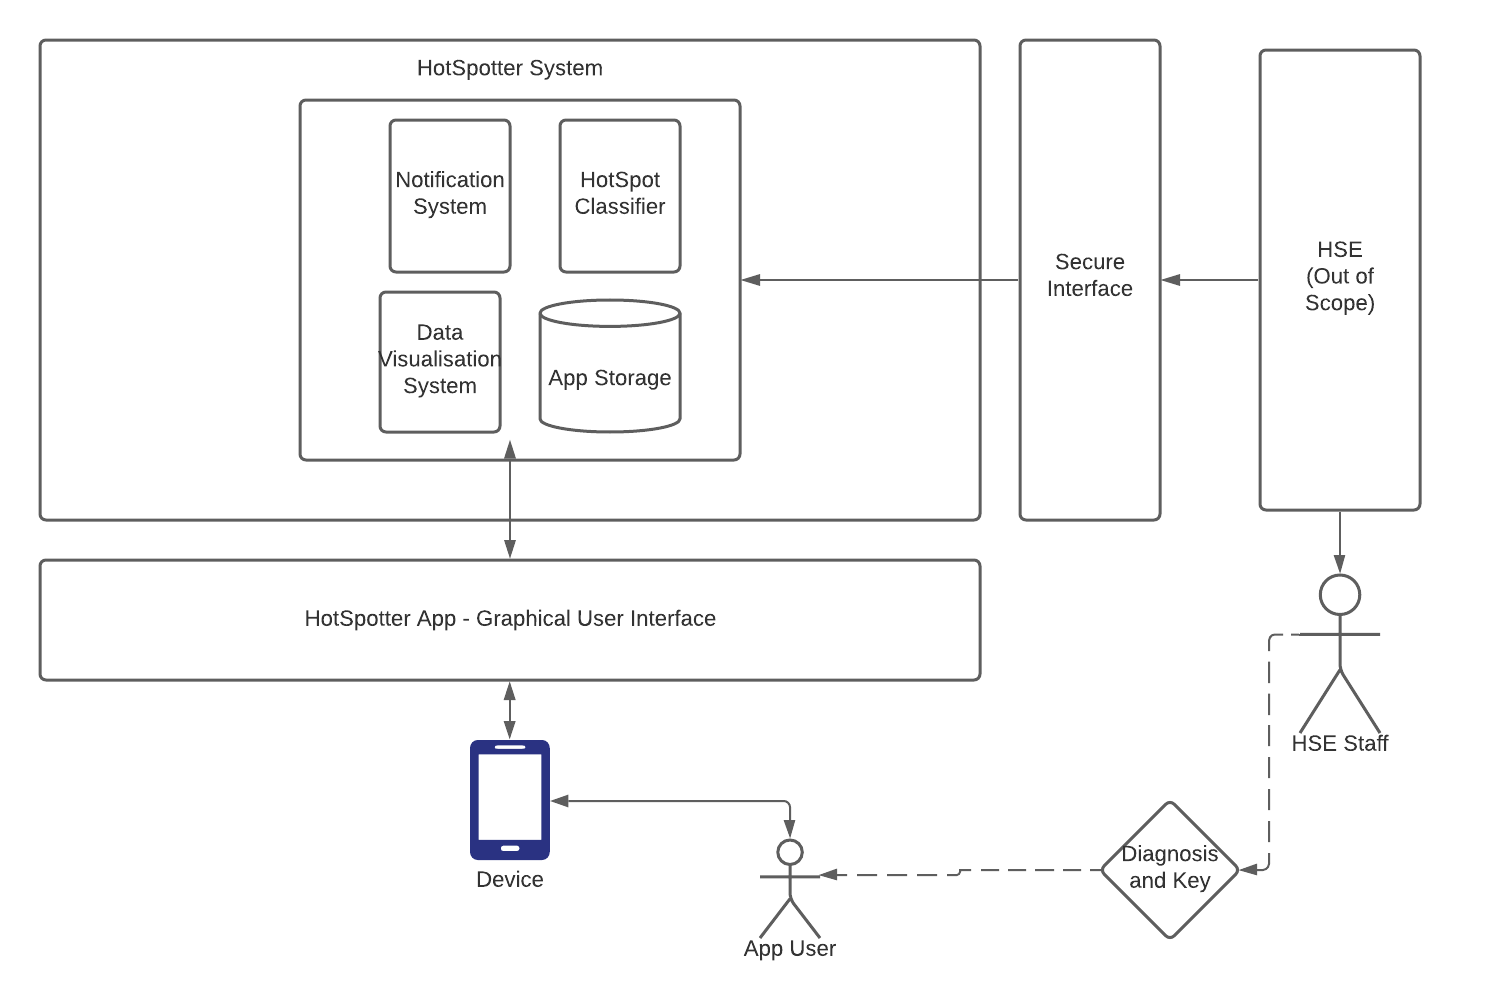
\includegraphics[width=0.9\linewidth]{InternalSystemComponents}
	\caption{The Model}
	\label{fig:System Components and Interfaces}
\end{figure}

\pagebreak
\section{System Interfaces}\label{SysInterface}
The following section details the various interfaces for the HotSpotter app.

\subsection{User Interface}\label{Interfaces}
This section details the interfaces between the user and the application.
\begin{itemize}
	\item A user will access and interact with the mobile application through a graphical user interface.
	\item A user will navigate around the application using touch or, if enabled by the user at a device level, voice commands.
	\item A user should be presented with a default homepage.
	\item All pages should be able to navigate to the Hotspot Page, the Contact Tracing Page, the Update Page, the Inbox Page, and the Settings Page.
	\item All pages should be intuitively navigatable to the user through the use of visual cues such as arrows, checkboxes, font headings.
	\item All pages should be responsive to the user.
	\item All pages must be available in English and Irish.
	\item All pages should be structured in a logical and consistent manner.
	\item All pages should use consistent font, styling, visual cues, and colouring.
	\item Push notifications and in-inbox messaging should conform to the styling of the application.
	\item All pages should have colour-blind friendly colour scheme customisation available.
	\item All visualisations and graphics should be labelled clearly and appropriately with axes, headers, units, and any other information appropriate for the accurate consumption of the information conveyed.
	\item The copy of the app should be written with minimal complexity.
	\item All interactions with opt-ins must be preserved.
\end{itemize}
A wireframe of the application detailing the expected level of connectivity between pages \href{https://www.fluidui.com/editor/live/project/p_5m9EtaKvry2LGyTzKWLHsE64PqSvu3rX}{here} and in Appendix \ref{wireframe}


\subsection{Hardware Interfaces}\label{HardInterface}
As this is a mobile application, the app will need:
\begin{itemize}
	\item A modern device and commonly used operating system to run.
	\item A device with appropriate technological capability to handle the implementation of contact tracing features and location services.
\end{itemize}
 
\subsection{Software Interfaces}\label{SoftInterface}
This section details software interfaces required for the running of the app. There are no explicit interfaces required, however some interface will be needed with the HSE's data for the retrieval of valid diagnostic keys and COVID19 updates.

\subsection{Communications Interfaces}\label{CommsInterface}
The app is required to be able to provide alerts to users.
\begin{itemize}
	\item For users opted in, push notifications are to display lock screen alerts and inbox alerts.
	\item For users opted out, only in-app inbox alerts are to be provided to users.
\end{itemize}

\subsection{Memory Constraints}\label{MemoryConstraints}
There are no explicit memory constraints.

\subsection{Operations}
There are no explicit operational requirements.


\subsection{Site Adaptation Requirements}
The HSE will develop the following data flows from their system to HotSpotter's and make any necessary changes needed to accomodate these:
\begin{itemize}
	\item Diagnostic Key Automated Data Transfer to enable the recording of verified diagnosed user reports in a format appropriate to allow for the population of HotSpotter's data tables and to exclude medical facilities from hotspot detection.
	\item COVID-19 Update Information Data Transfer to enable the display of the latest COVID-19 updates and statuses in a format to display to users in the app.
\end{itemize}

\section{Product Functions}\label{ProductFunction}
This section details the key functions of the product.

\subsection{Identify and Visually Display Hotspots}
The application should be able to identify hotspots as defined in \ref{Defn} and display this graphically on a map with hotspots nearest the user appearing first and the most significant hotspots in terms of incidence prevalence should be highlighted.

The hotspot identification process flow is detailed in figure \ref{hotflow}
\begin{figure}[H]
	\centering
	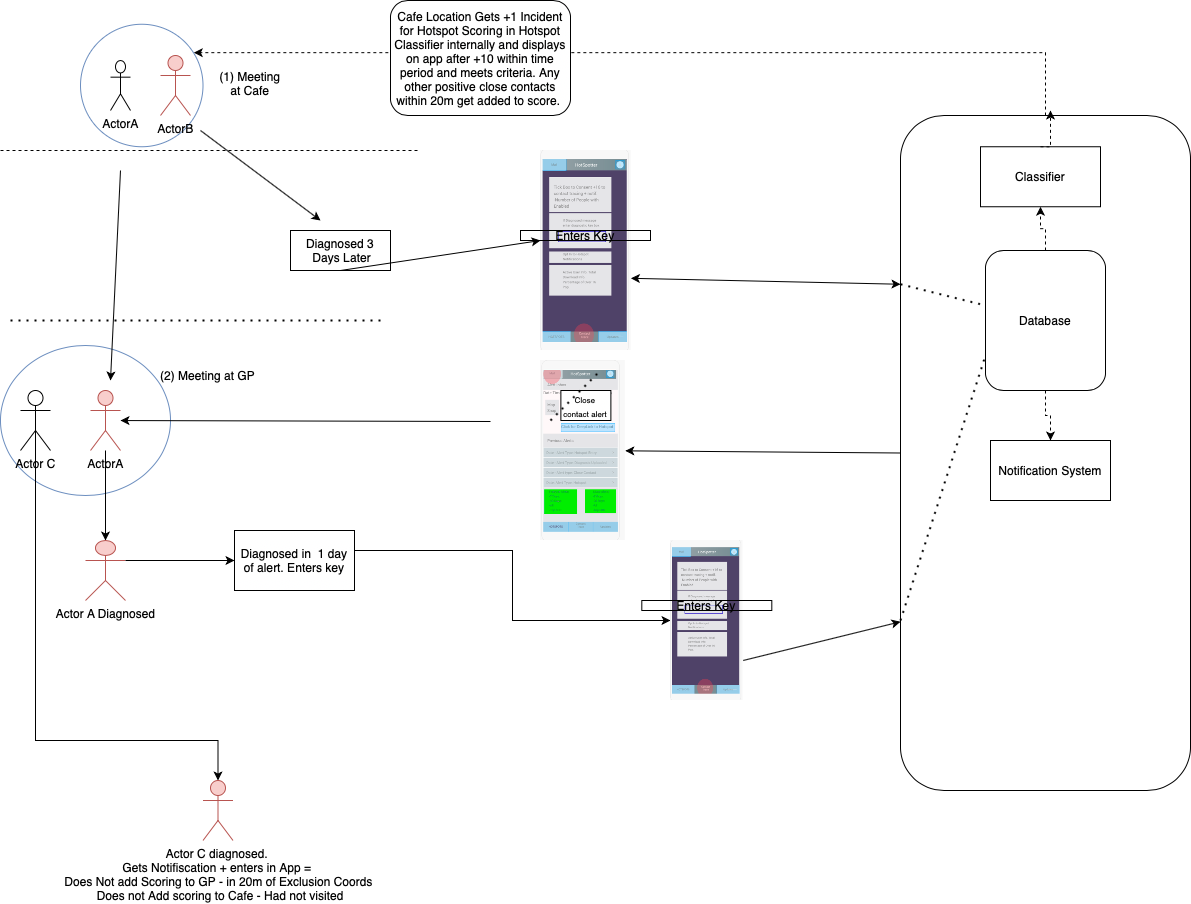
\includegraphics[page=1, width=0.95\linewidth]{COMP30830-HotSpotClassifierFlow}
	\caption{Hotspot Identification Flow}
	\label{hotflow}
\end{figure}

\subsection{Display additional Hotspot Metrics}
The application should be able to provide a graphical view of when the hotspot is most likely to produce close contacts, put the hotspot in context of other hotspots in the nation, and display the history of the hotspot over time.

\subsection{Allow the searching of a Hotspot}
The application should allow the user to search a location and identify hotspots nearby and view the same information as if the user was located their.

\subsection{Contact Tracing}
The application should allow the user to begin contact tracing and notifying them or others if they are close contacts.

\subsection{Notification}
The app should feature both push notifications and in-app inbox messaging. When a user enters a hotspot, they should be alerted to put on their mask. When a user is a close contact, they should receive a notification to get tested for COVID-19. The user should be able to view their notification history.

\subsection{Confirm Diagnosis}
The app should allow users to self-report a diagnosis of COVID-19, and validated their report via a diagnostic key provided to them by their doctor and alert their close contacts to get tested.

\subsection{COVID-19 Updates}
The app should have a page displaying information provided by the HSE including stats about COVID, news on COVID, and the county split of COVID users.

\subsection{Notification Retention}
The application should retain history of notifications received and provide the user with information on how many updates of a hotspot warning or close contact warning they've received

\subsection{Privacy Focused and Transparent}
The application should be transparent in what data is held to the user, and should have all data anonymised to increase trust and compliance in the application.

\subsection{Accessible}
The application should be designed with accessibility in mind and adjustable to the needs of a wider user base. 

\section{User Characteristics}

The intended user of the application is to be the population of Ireland. As such, users vary in educational level, experience, and technical expertise from low-expertise to high-expertise, with a range of accessibility requirements from language to assistive technological needs. The app should be designed with accessibility in mind to remove barriers of use. This has an impact on the user interface referred to in \ref{Interfaces} and an impact on the requirements outlined in \ref{Requirements}
Describe those general characteristics of the intended users of the product including educational level, experience, and technical expertise.  Do not state specific requirements but rather provide the reasons why certain specific requirements are later specified in section \ref{Requirements}. \\
\\
For this application, there are no specific user roles outside of user.\\
\\
Typical user journeys for app users include:\\
\\
Scenario 1
\begin{enumerate}
	\item User downloads app onto their device.
	\item User consents to notifications and contact tracing features.
	\item User plans to make journey and sees that it is a hotspot.
	\item User views more information on the hotspot and notes that on today's day of the week COVID contacts are twice as high as other dates.
	\item User makes essential journey in mask and is conscious of maintaining social distancing.
	\item User makes detour on journey on way home and unbeknowingly enters a hotspot. 
	\item The application alerts the user of a hotspot.
	\item User ensures mask is active.
\end{enumerate}
Scenario 2
\begin{enumerate}
	\item User has been using app and receives a close contact alert.
	\item User clicks app notification and is taken to the region where the close contact took place.
	\item User notices area is a hotspot and there were therefore many users with COVID at the time user visited.
	\item User schedules a GP appointment and alerts them of the close contact warning and hotspot status.
	\item GP immediately tests for COVID and user is diagnosed.
	\item User reports their diagnosis by entering their diagnostic key into the app.
	\item Close contacts of user are alerted.
\end{enumerate}
Scenario 3 
\begin{enumerate}
	\item User is interested in identifying how their business is doing in maintaining social distancing requirements.
	\item User checks their region in the HotSpotter.
	\item User looks at more info on the region and observes region where there business is located has been a hotspot twice in the last thirty days.
	\item User informs their staff members of this and ensures that all staff members are conscious of risk of COVID-19.
\end{enumerate}
Scenario 4
\begin{enumerate}
	\item User is considering visiting a local cafe to meet up with friends.
	\item User has at-risk relatives within their household.
	\item User checks the status of the area and notices that it has been a hotspot multiple times over the course of the last six months.
	\item User decides the journey is non-essential and decides not to go on trip.
\end{enumerate}

\section{Constraints}
The following constraints are present in the system design:

\subsection{Regulatory Policies}
The system should comply with GDPR and the Data Protection Act.

\subsection{Hardware Limitations}
The system should be able to run on modern mobile hardware and operating systems.

\subsection{Interfaces}
The system will need to interface with the HSE's system (outside the scope of this SRS) for the retrieval of data.

\subsection{Audit Info}
The system will need to capture and record user's consent options and changes.

\subsection{Reliability}
The system will need to run at all times and should be able to run efficiently without downtime or performance degradation even with a large user base. The information in the app should be kept up-to-date and trust-worthy.

\subsection{Adjustable}
The definition of a hotspot needs to be maintainable as the COVID-19 pandemic develops.


\section{Assumptions and Dependencies}
It is assumed within the SRS that all modern smartphones will be capable of running the application, and that the features outlined are feasible to modern smartphones. If a smartphone does not have the performance capacity capable of running some of the features, or OS releases impact some of the dependencies, it is understood that the user may not have the expected experience. Similarly, it's assumed that the contact tracing feature is platform agnostic in that it does not matter which operating system or device a user has, it is still capable of engaging in contact tracing with devices' with other specifications. If this is not the case, and there are OS specific dependencies, the application design will need to be adjusted to facilitate cross-platform contact tracing.

\section{Apportioning of Requirements}
Features have been split between Core, High, Medium, and Low priority as outlined by the client. Core features are features which are expected and anticipated to be available within the MVP release if full feature-inclusion for the release deadline cannot be met. The final undelivered features should be prioritised based on the ranking of High, Medium, and Low.


\chapter{Specific Requirements}\label{Requirements}


\section{External Interfaces}
This section details the external systems feeding into the HotSpotter application.
\begin{figure}[H]
	\centering
	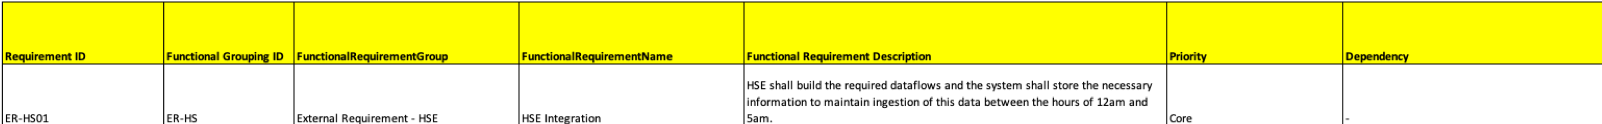
\includegraphics[page=1, width=0.95\linewidth]{COMP30830-ExternalRequirements}
	\caption{External Requirements Table}
	\label{FR}
\end{figure}

\section{User Interface Requirements}\label{UXReq}
This section details the requirements for the user interface. These requirements are designed to compliment and add context to the FluidUI wireframe located \href{https://www.fluidui.com/editor/live/project/p_5m9EtaKvry2LGyTzKWLHsE64PqSvu3rX}{here}\\
\begin{figure}[H]
	\centering
	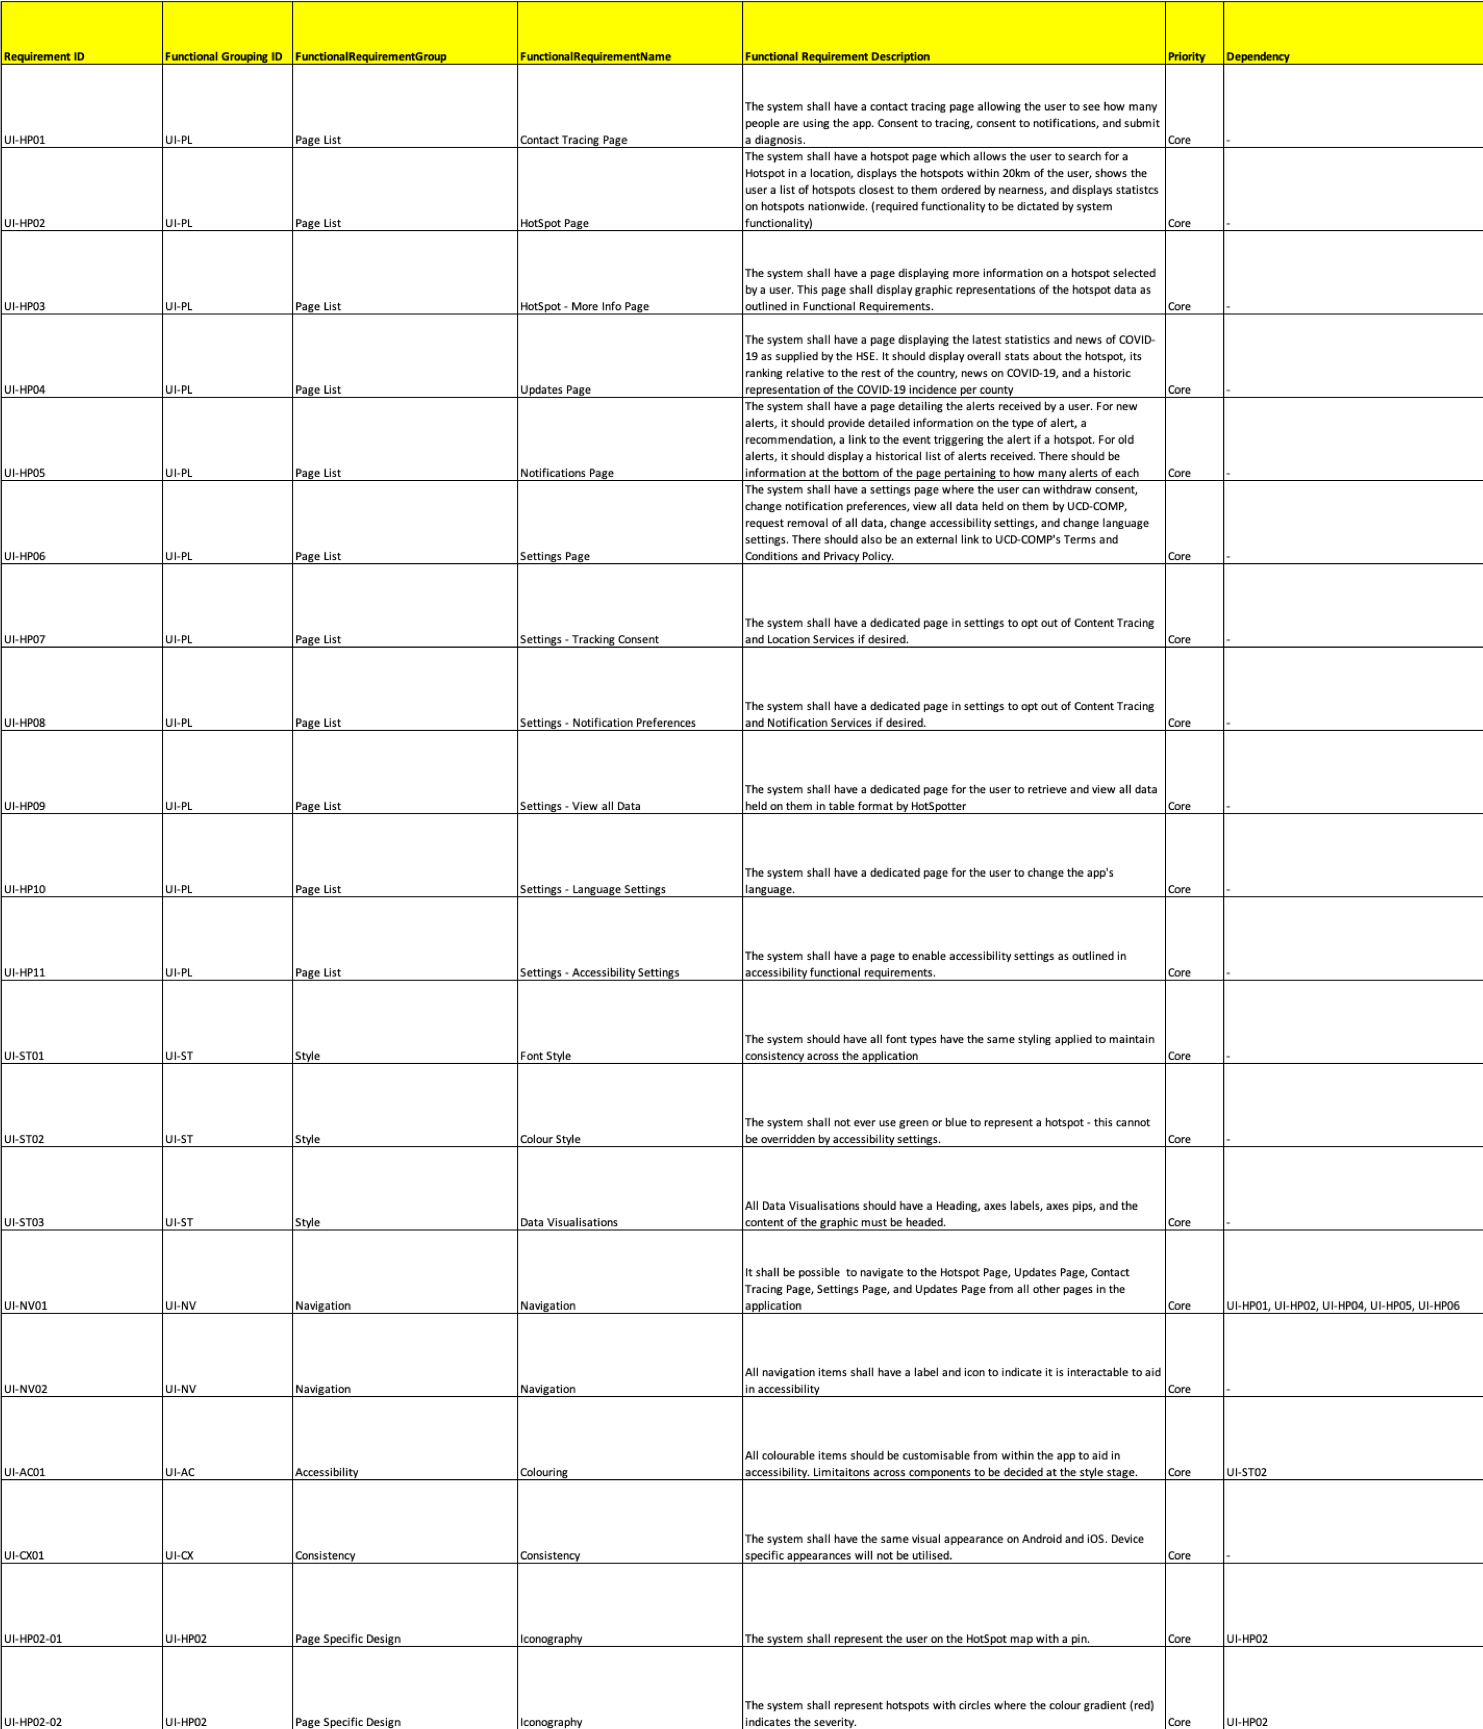
\includegraphics[page=1, width=0.95\linewidth]{COMP30830-UserRequirements}
	\caption{UX Requirements Table}
	\label{UXR}
\end{figure}


\section{System Features}
The functional requirements of the application have been structured using a feature organisation structure, and features have been grouped according to similarity. The functional requirements of the application has been designed with the specificity and accuracy feasible at this stage, however design details of these functions are left to the expertise of the UCD-COMP development team for implementation.\\
\\
\subsection{HotSpot Features}

\subsubsection{HotSpot Definition}
As discussed in \ref{Defn}, following the CDC definition of a hotspot adjusted to the Irish market and app usage as outlined by the HSE, a hotspot shall be a region where
\begin{itemize}
	\item The region has a radius of 20m and does not intersect within 20m of a hospital, a HSE registered general practitioner's office.
	\item  $\geq 10$ new close-contacts who visited the area tested positive for COVID-19 within $7$ days of receiving a close-contact alert.
	\item an increase in the most recent $7$-day COVID-19 incidence of close-contacts testing positive for COVID-19 within $7$ days of a close-contact alert, over the preceding $7$-day incidence of close-contacts testing positive for COVID-19 within $7$ days of a close-contact alert.
	\item a decrease of $\leq 60\%$ or an increase in the most recent $3$-day COVID-19 incidence of close-contacts testing positive for COVID-19 within $7$ days of a close-contact alert over the preceding $3$-day incidence of close-contacts testing positive for COVID-19 within $7$ days of a close-contact alert. 
	\item the ratio of $7$-day incidence of close-contacts testing positive for COVID-19 within $7$ days of a close-contact alert/$30$-day incidence of close-contacts testing positive for COVID-19 within $7$ days of a close-contact alert exceeds $0.31$. In addition, hotspots must have met at least one of the following criteria: 
	\begin{itemize}
		\item[$-$] $\geq 60\%$ change in the most recent 3-day COVID-19 incidence of close-contacts testing positive for COVID-19 within $7$ days of a close-contact alert.
		\item[$-$]$\geq 60\%$ change in the most recent 7-day incidence of close-contacts testing positive for COVID-19 within $7$ days of a close-contact alert.
	\end{itemize}
\end{itemize}
The implementation details of this definition is left up to the development and design team and the classification of areas into hotspots shall be a key requirement of the application.\\
\\
The severity of the hotspot should by the $7$-day incidence of close-contacts testing positive for COVID-19 within $7$ days of a close-contact alert from contact with a user in that hotspot radius.

\subsection{System Features}
This section details the functional system requirements of the app.
\subsubsection{HotSpot Features}
This section details functional requirements concerning the hotspot features.
\begin{figure}[H]
	\centering
	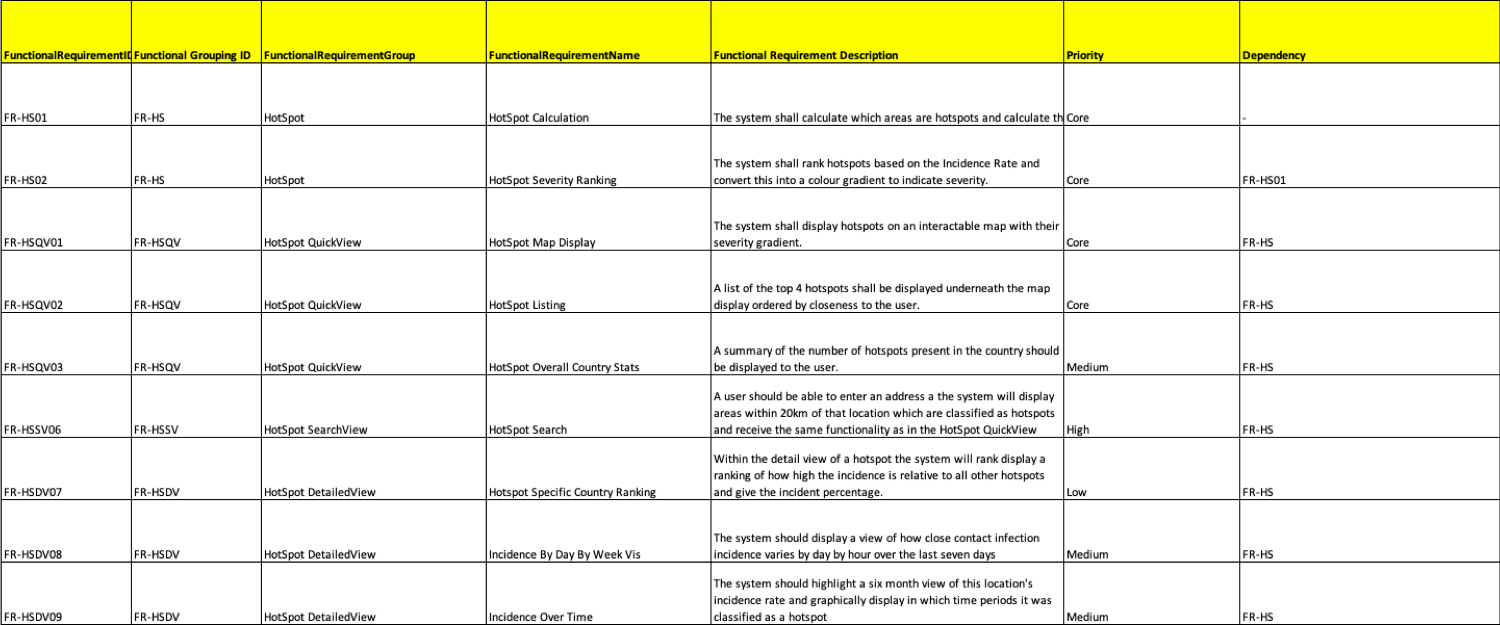
\includegraphics[page=1, width=0.95\linewidth]{COMP30830-FunctionalRequirements-Hot}
	\caption{Functional Requirements Table - HotSpots}
	\label{FR}
\end{figure}

\subsection{Contact Tracing And Notification Features}
This section details functional requirements concerning the contact tracing and notification features.
\begin{figure}[H]
	\centering
	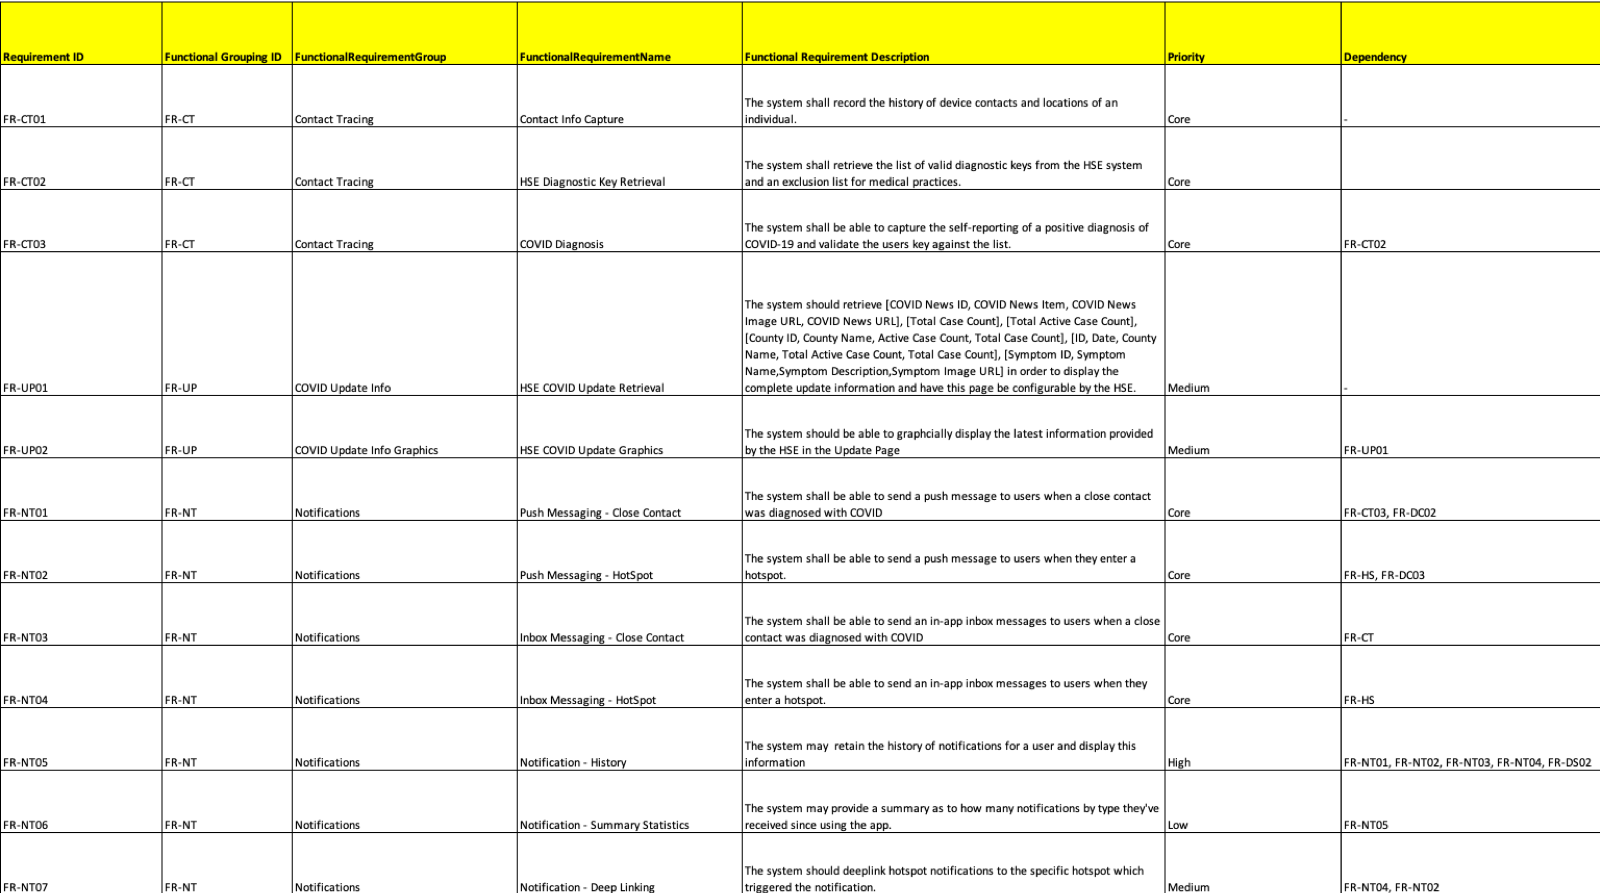
\includegraphics[page=1, width=0.95\linewidth]{COMP30830-FunctionalRequirements-CT}
	\caption{Functional Requirements Table - Contact Tracing and Notifications}
	\label{FR}
\end{figure}

\subsection{Privacy and Accessibility Features}
This section shall detail functional requirements surrounding privacy and accessibility features. These features are considered functional as there are functional requirements underlying the inclusion of these features necessitating that they are available within the app before launch.
\begin{figure}[H]
	\centering
	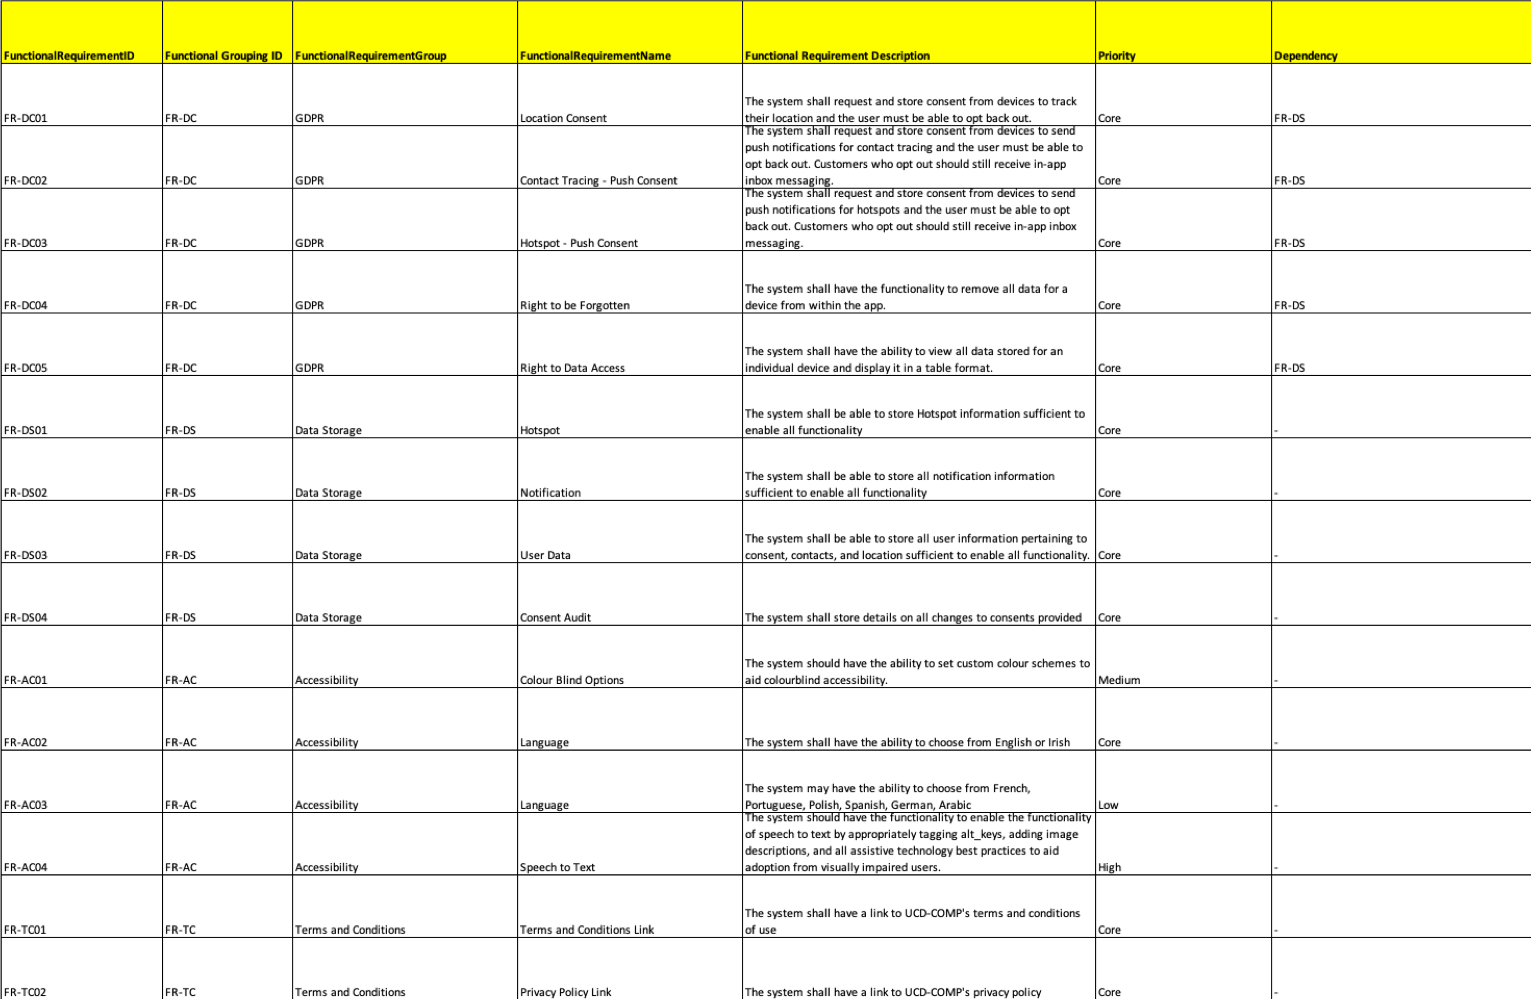
\includegraphics[page=1, width=0.95\linewidth]{COMP30830-FunctionalRequirements-Acc}
	\caption{Functional Requirements Table - GDPR, Data Storage, Accessibility}
	\label{FR}
\end{figure}



\section{Performance Requirements}
This section details some key performance requirements for the app.
\begin{figure}[H]
	\centering
	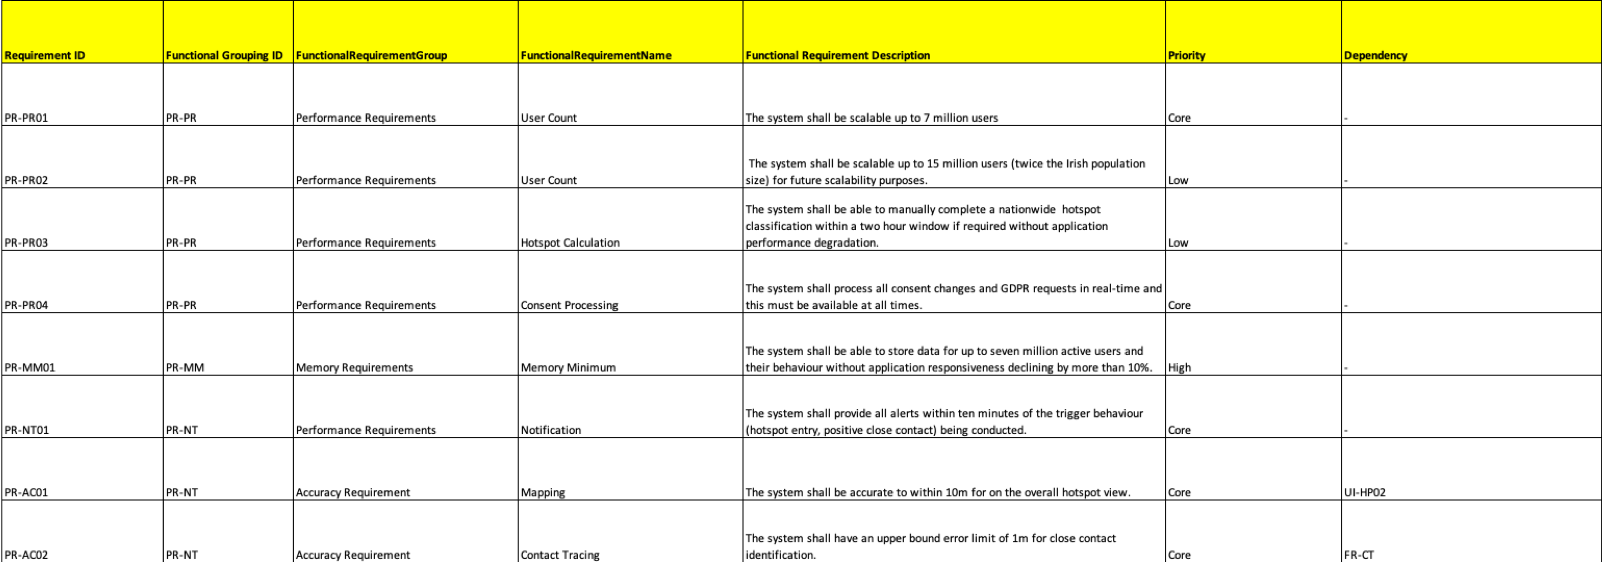
\includegraphics[page=1, width=0.95\linewidth]{COMP30830-PerformanceRequirements}
	\caption{Performance Requirements Table}
	\label{PR}
\end{figure}

\section{Logical Database Requirements}
While data must be stored into a database for the functionality of the app, there is no explicit requirements on what the database structure or representation must look like so long as the other requirements are fulfilled.


\section{Design Constraints Requirements}
This section outlines some design constraints which must be followed by the application.

\subsection{Standard Compliance}
This section details some standards which the app must be compliant with.\begin{figure}[H]
\centering
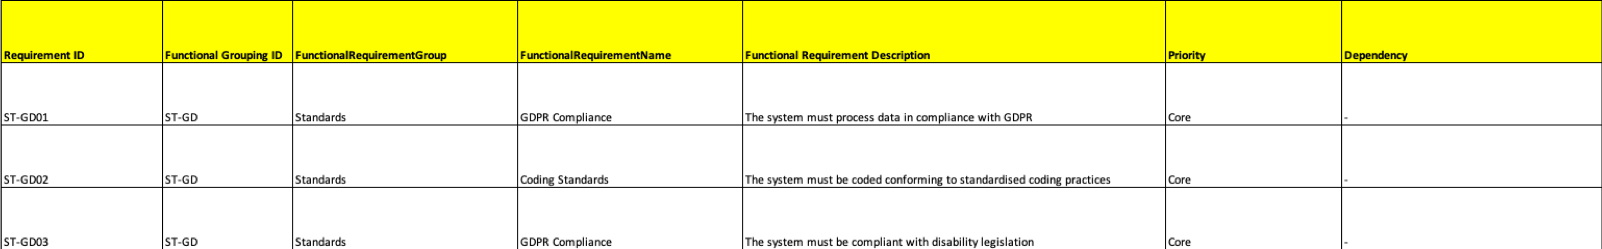
\includegraphics[page=1, width=0.95\linewidth]{COMP30830-StandardsRequirements}
\caption{Standard Compliance Requirements Table}
\label{DR}
\end{figure}
The requirement concerning conforming to standardised coding practices includes the need to pass release requirements for app distribution channels.

\section{Software System Attributes}
This section details some attributes of the software system not otherwise covered in previous requirement sections.
\\

\subsection{Reliability}
This section covers some of the reliability requirements which are needed for the application.
\begin{figure}[H]
	\centering
	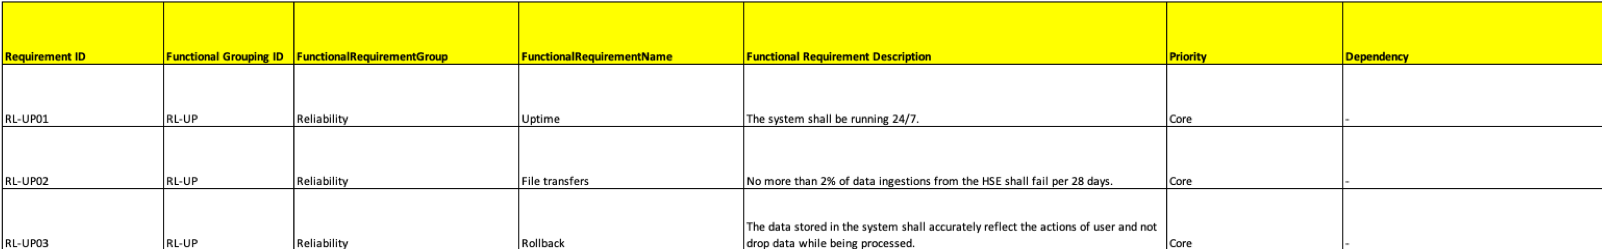
\includegraphics[page=1, width=0.95\linewidth]{COMP30830-ReliabilityRequirements}
	\caption{Reliability Requirements Table}
	\label{RR}
\end{figure}


\subsection{Security}
This section details some of the security requirements for the HotSpotter application.
\begin{figure}[H]
	\centering
	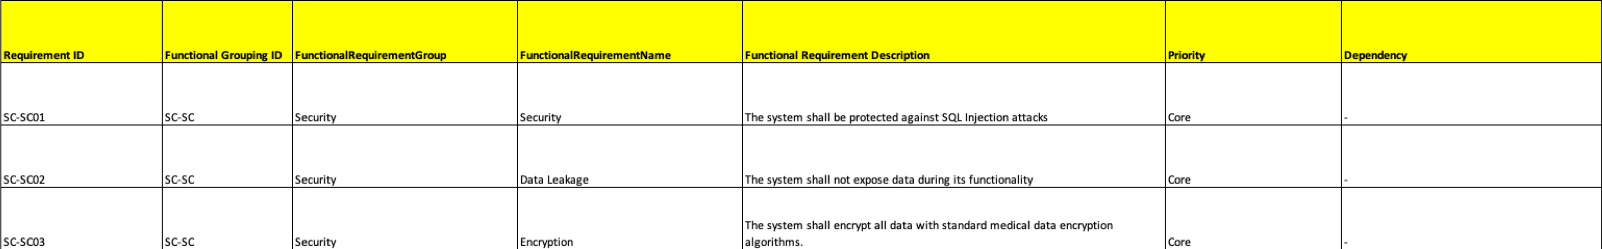
\includegraphics[page=1, width=0.95\linewidth]{COMP30830-SecurityRequirements}
	\caption{Security Requirements Table}
	\label{SR}
\end{figure}


\subsection{Maintainability}
This section covers some of the requirements surrounding maintainability of the HotSpotter Application.
\begin{figure}[H]
	\centering
	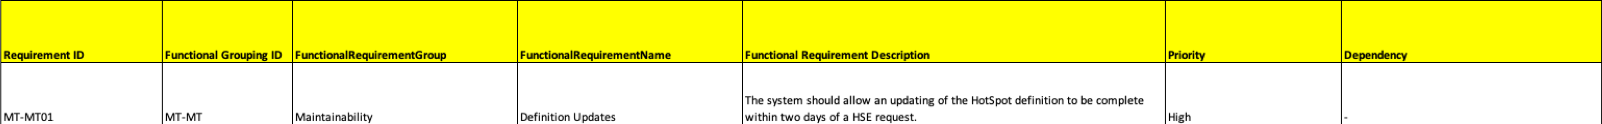
\includegraphics[page=1, width=0.95\linewidth]{COMP30830-MaintainRequirements}
	\caption{Maintain Requirements Table}
	\label{MR}
\end{figure}


\subsection{Portability and Hardware}
This section details requirements of the HotSpotter
application for the purpose of porting the application to various other systems of software or hardware, and the associated hardware requirements. \\
\begin{figure}[H]
	\centering
	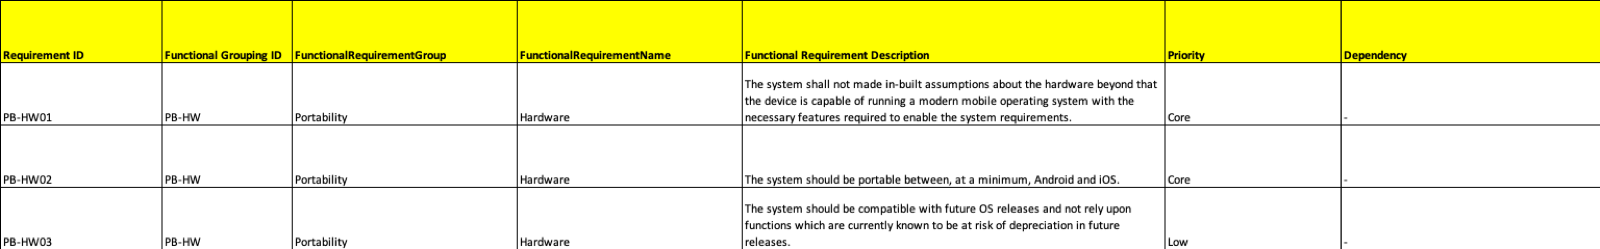
\includegraphics[page=1, width=0.95\linewidth]{COMP30830-PortabilityRequirements}
	\caption{Portability Requirements Table}
	\label{PortR}
\end{figure}



\section{Change Request Process}
The change request process shall be defined as follows:
\begin{enumerate}
	\item The product sponsor shall submit a file containing specific details of the change request to the UCD-COMP product owner. 
	\item The change request will be reviewed and discussed by UCD-COMP.
	\item At the end of the current sprint, a Change Advisory Board meeting will be called involving the product sponsor, product owner, and any additional participants who may be required to work on the change.
	\item An agreement will be made on the scope of the change and any additional cost implication of the change. 
	\item A Statement of Work will be prepared by UCD-COMP detailing the requirement changes, cost implications, and effort requirements
	\item The Statement of Work will be signed off by the product owner and product sponsor and added into the SRS appendix.
	\item The change will be implemented into the SRS document.
	\item The revised SRS draft will be signed off by both the product owner and product sponsor.
\end{enumerate}

\section{Document Approvals}
The document must be approved by the product owner and product sponsor before ebing confirmed as final.


\begin{center}
	\begin{tabular}{|c|c|c|}
		\hline
		Name & Role & Date \\
		\hline
		Gregory House & HSE Product Sponsor & 2020-02-14\\
		\hline
		 John Judge & UCD-COMP Product Owner & 2020-02-14 \\
		\hline
	\end{tabular}
\end{center}

\chapter{Appendix}

\subsection{New Zealand Privacy Commissioner Track and Trace App Comparison - 5th May 2020}\label{nz-rep}
The complete comparison of COVID-19 apps released in various locations as completed by the Privacy Commissioner of New Zealand\\
\begin{figure}[H]
	\centering
	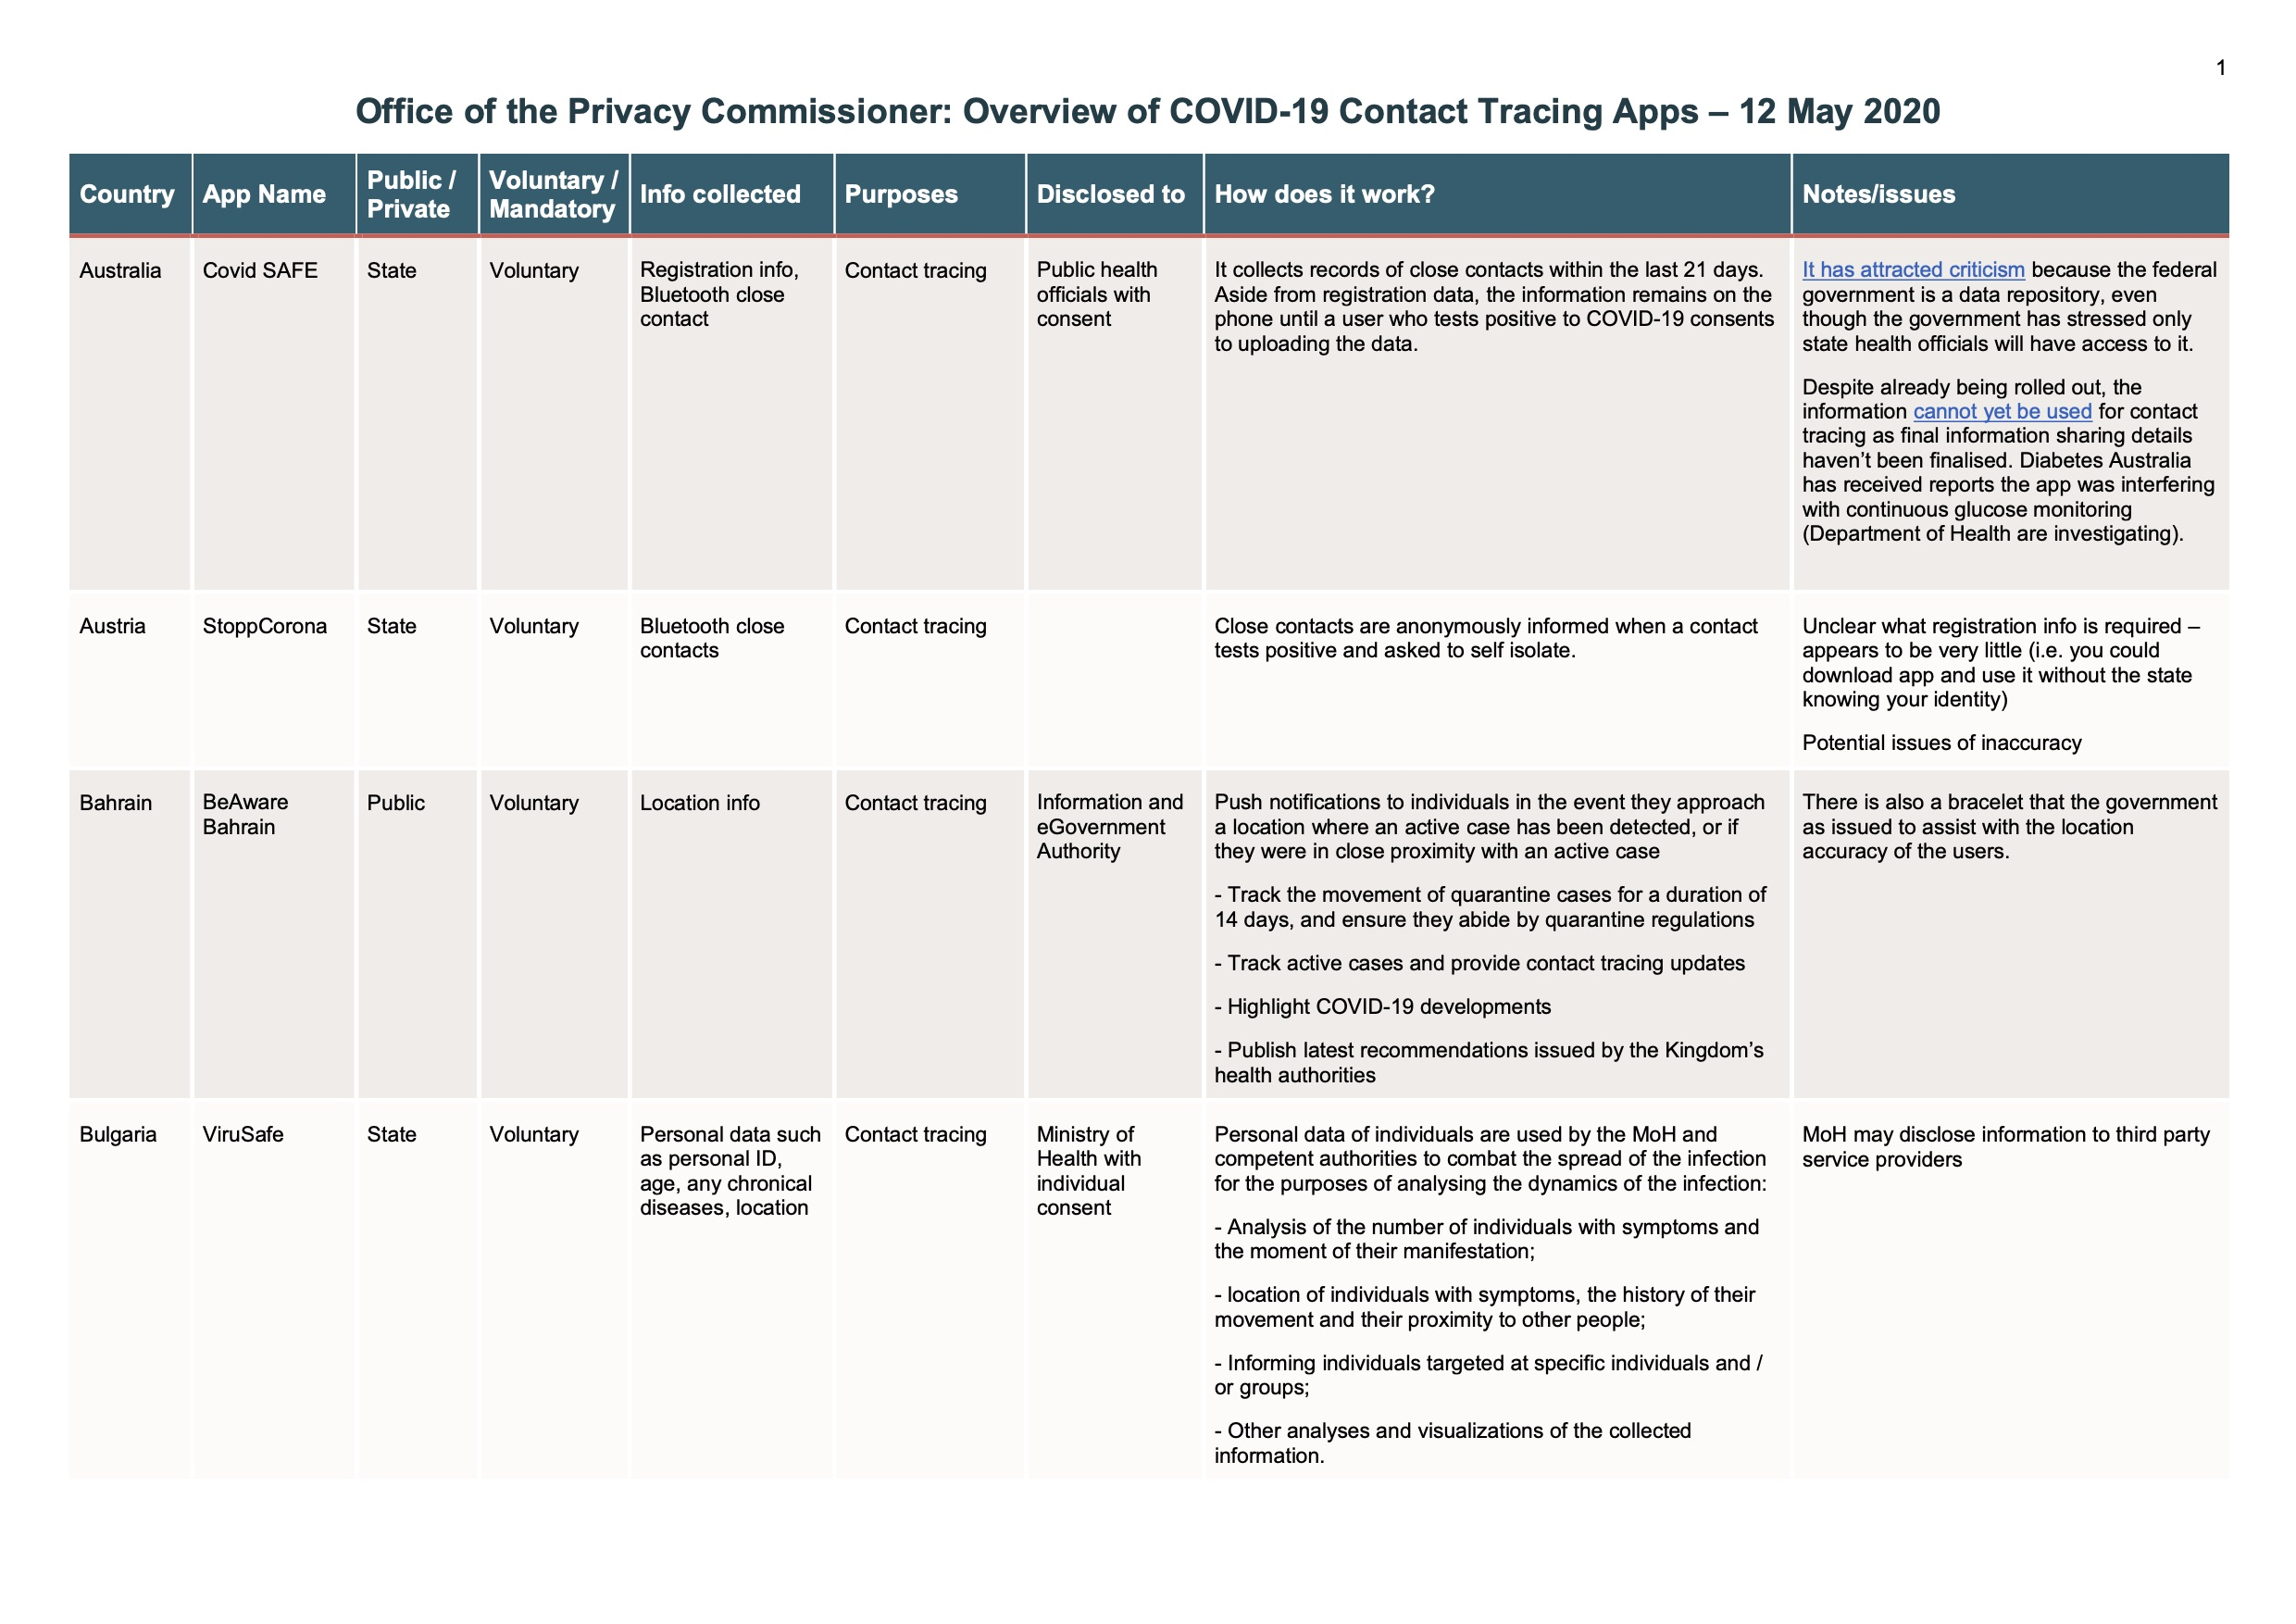
\includegraphics[page=1, width=0.9\linewidth]{2020-05-12-OPC-Comparison-of-COVID-19-Apps-colours}
	\caption{International App Comparison Page 1}
	\label{fig:1_2020-05-12-OPC-Comparison-of-COVID-19-Apps-colours}
\end{figure}

\begin{figure}[H]
	\centering
	\includegraphics[page=2, width=0.9\linewidth]{2020-05-12-OPC-Comparison-of-COVID-19-Apps-colours}
	\caption{International App Comparison Page 2}
	\label{fig:2_2020-05-12-OPC-Comparison-of-COVID-19-Apps-colours}
\end{figure}

\begin{figure}[H]
	\centering
	\includegraphics[page=3, width=0.9\linewidth]{2020-05-12-OPC-Comparison-of-COVID-19-Apps-colours}
	\caption{International App Comparison Page 3}
	\label{fig:3_2020-05-12-OPC-Comparison-of-COVID-19-Apps-colours}
\end{figure}

\begin{figure}[H]
	\centering
	\includegraphics[page=4, width=0.9\linewidth]{2020-05-12-OPC-Comparison-of-COVID-19-Apps-colours}
	\caption{International App Comparison Page 4}
	\label{fig:4_2020-05-12-OPC-Comparison-of-COVID-19-Apps-colours}
\end{figure}

\begin{figure}[H]
	\centering
	\includegraphics[page=5, width=0.9\linewidth]{2020-05-12-OPC-Comparison-of-COVID-19-Apps-colours}
	\caption{International App Comparison Page 5}
	\label{fig:5_2020-05-12-OPC-Comparison-of-COVID-19-Apps-colours}
\end{figure}

\begin{figure}[H]
	\centering
	\includegraphics[page=6, width=0.9\linewidth]{2020-05-12-OPC-Comparison-of-COVID-19-Apps-colours}
	\caption{International App Comparison Page 6}
	\label{fig:6_2020-05-12-OPC-Comparison-of-COVID-19-Apps-colours}
\end{figure}
\begin{figure}[H]
	\centering
	\includegraphics[page=7, width=0.9\linewidth]{2020-05-12-OPC-Comparison-of-COVID-19-Apps-colours}
	\caption{International App Comparison Page 7}
	\label{fig:7_2020-05-12-OPC-Comparison-of-COVID-19-Apps-colours}
\end{figure}

\begin{figure}[H]
	\centering
	\includegraphics[page=8, width=0.9\linewidth]{2020-05-12-OPC-Comparison-of-COVID-19-Apps-colours}
	\caption{International App Comparison Page 8}
	\label{fig:8_2020-05-12-OPC-Comparison-of-COVID-19-Apps-colours}
\end{figure}
\begin{figure}[H]
	\centering
	\includegraphics[page=9, width=0.9\linewidth]{2020-05-12-OPC-Comparison-of-COVID-19-Apps-colours}
	\caption{International App Comparison Page 9}
	\label{fig:9_2020-05-12-OPC-Comparison-of-COVID-19-Apps-colours}
\end{figure}
\begin{figure}[H]
	\centering
	\includegraphics[page=10, width=0.9\linewidth]{2020-05-12-OPC-Comparison-of-COVID-19-Apps-colours}
	\caption{International App Comparison Page 10}
	\label{fig:10_2020-05-12-OPC-Comparison-of-COVID-19-Apps-colours}
\end{figure}


\subsection{App Wireframe}\label{wireframe}
This section details the connectivity and wireframe of the application. Elements of this wireframe not outlined explicitly as requirements should not be interpretted as design decisions.

\begin{figure}[H]
	\centering
	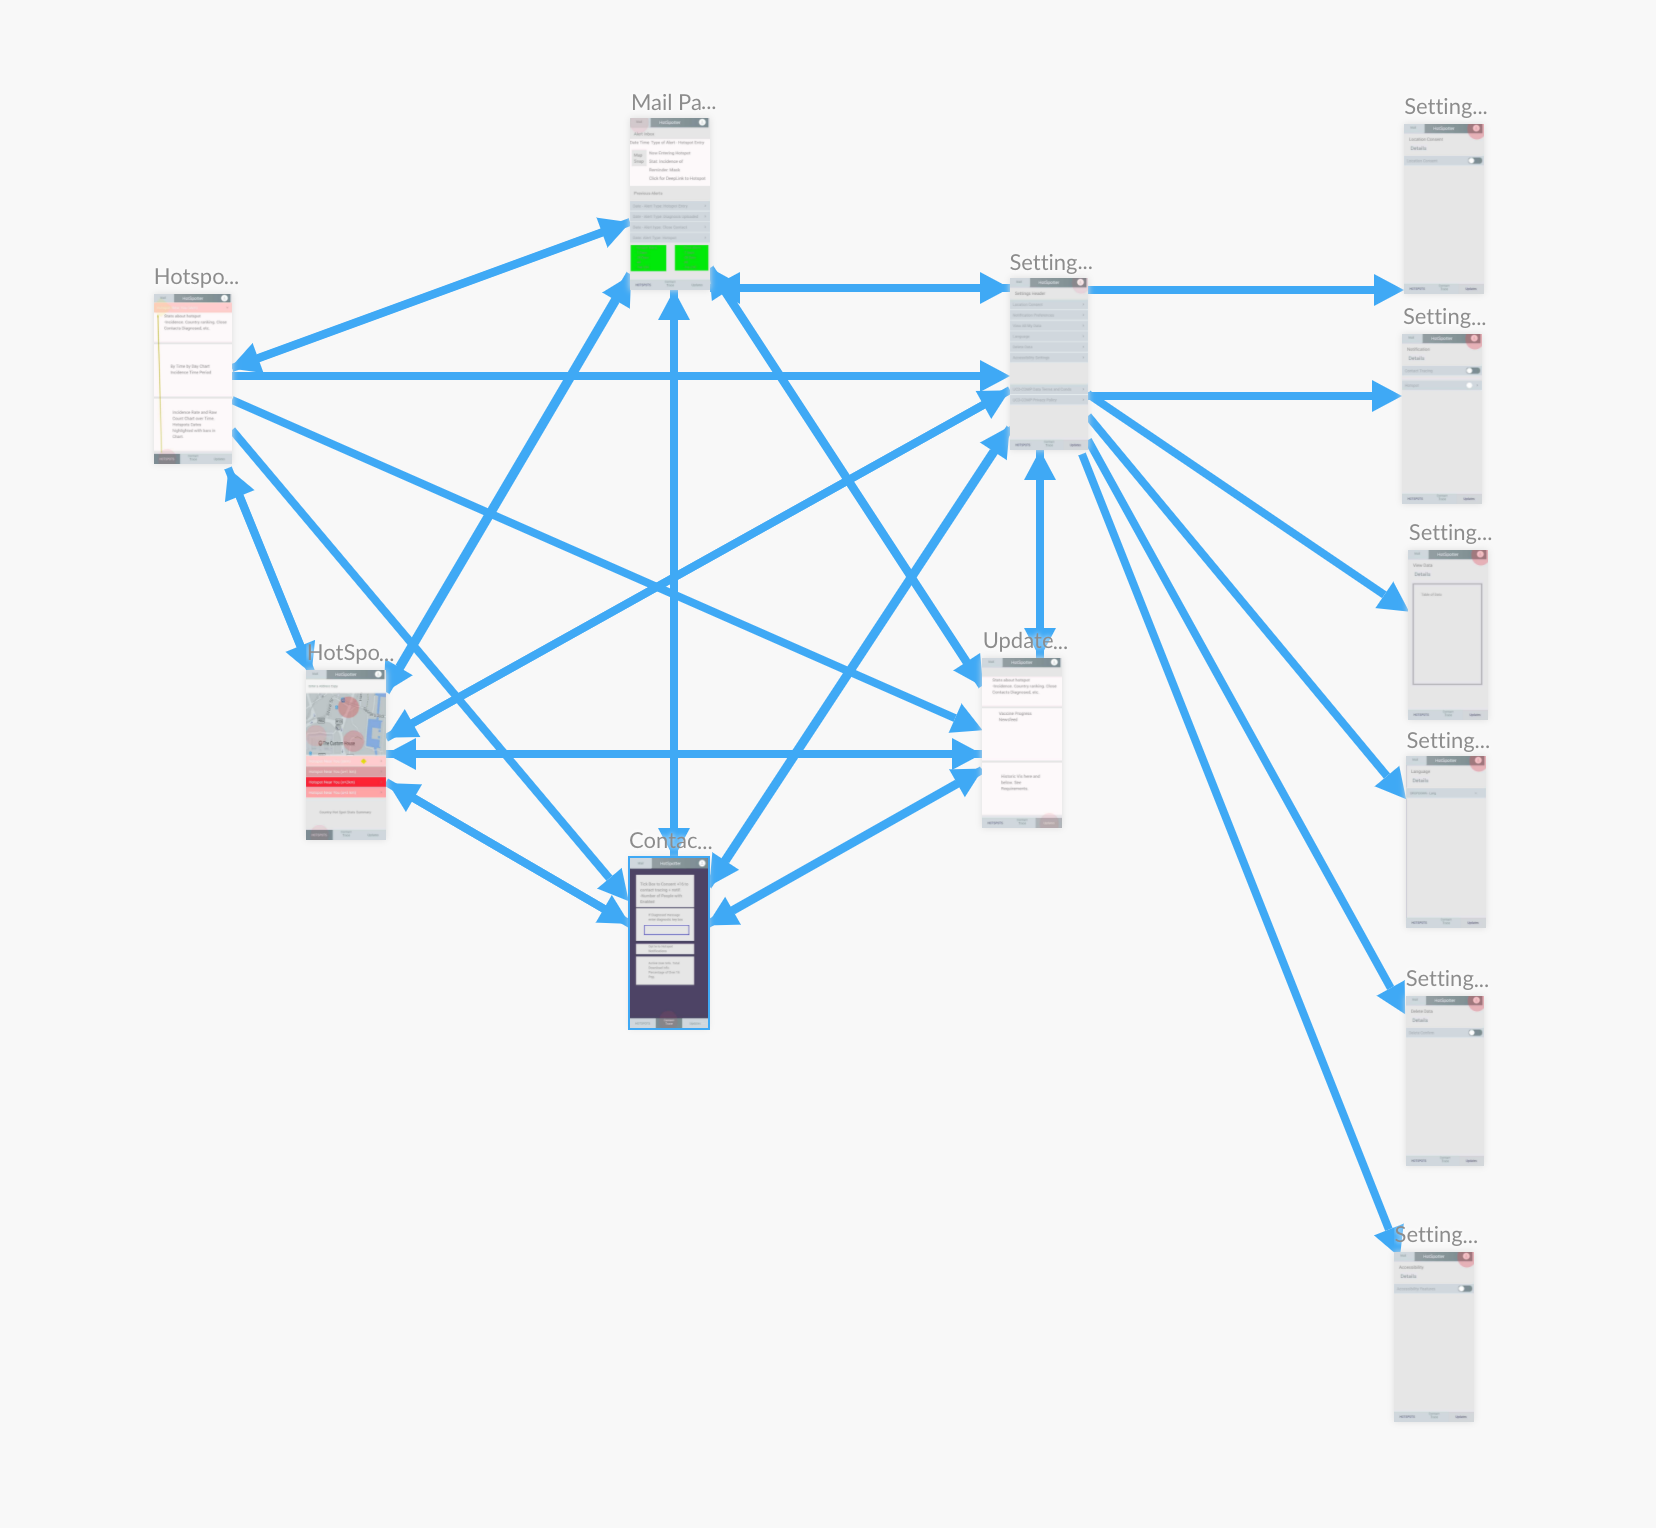
\includegraphics[page=1, width=0.9\linewidth]{COMP30830-AppUIWireFrame}
	\caption{App User Interface Connectivity - For diagram Connections between the Settings pages and the other pages have been removed however should be present in the final design}
	\label{UIConnectivity}
\end{figure}

\begin{figure}[H]
	\centering
	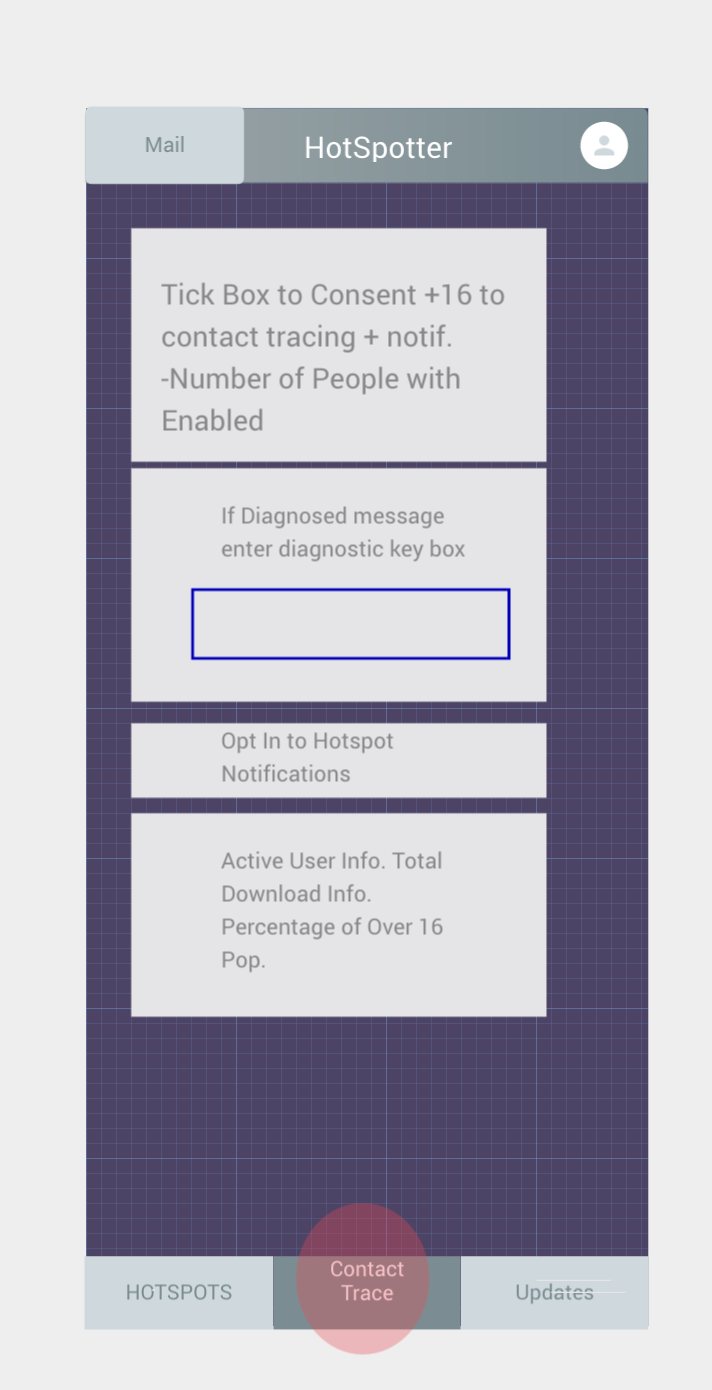
\includegraphics[page=1, width=0.9\linewidth]{COMP30830-Contact}
	\caption{Main Page - Contact Tracing}
	\label{Connectivity}
\end{figure}


\begin{figure}[H]
	\centering
	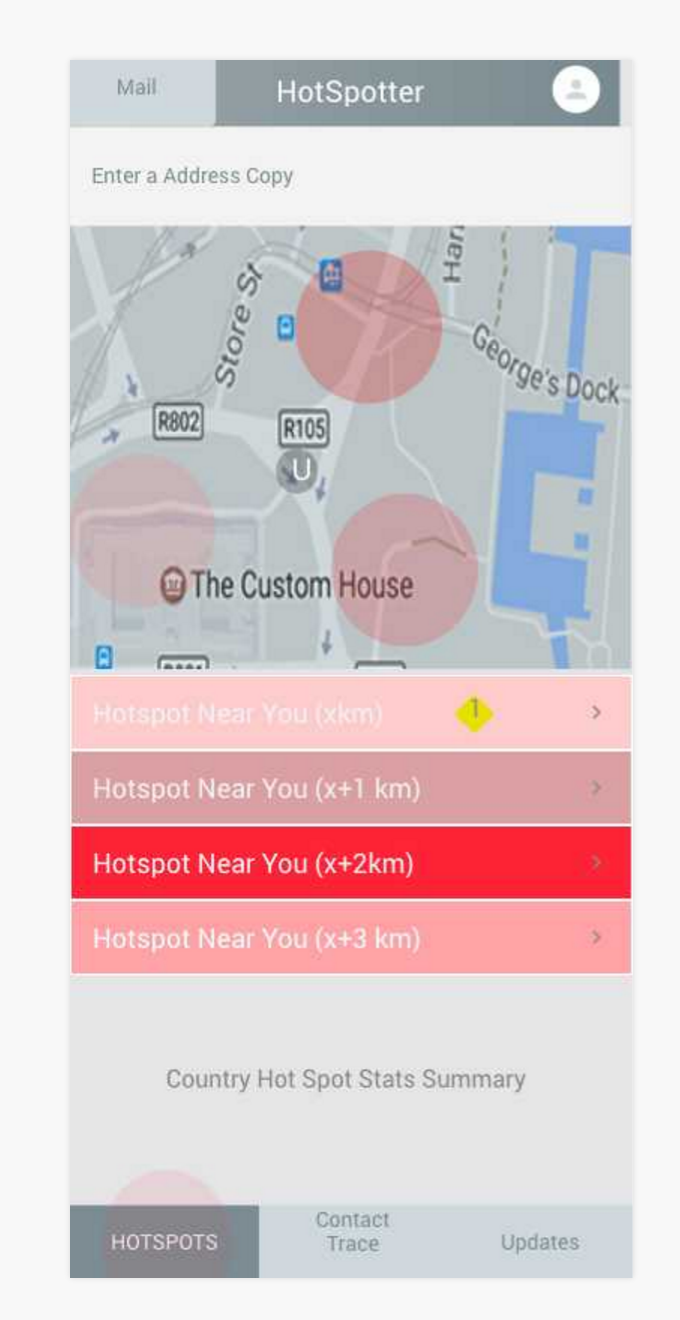
\includegraphics[page=1, width=0.9\linewidth]{COMP30830-Hotspots}
	\caption{Main Page - HotSpots}
	\label{HotSpots}
\end{figure}


\begin{figure}[H]
	\centering
	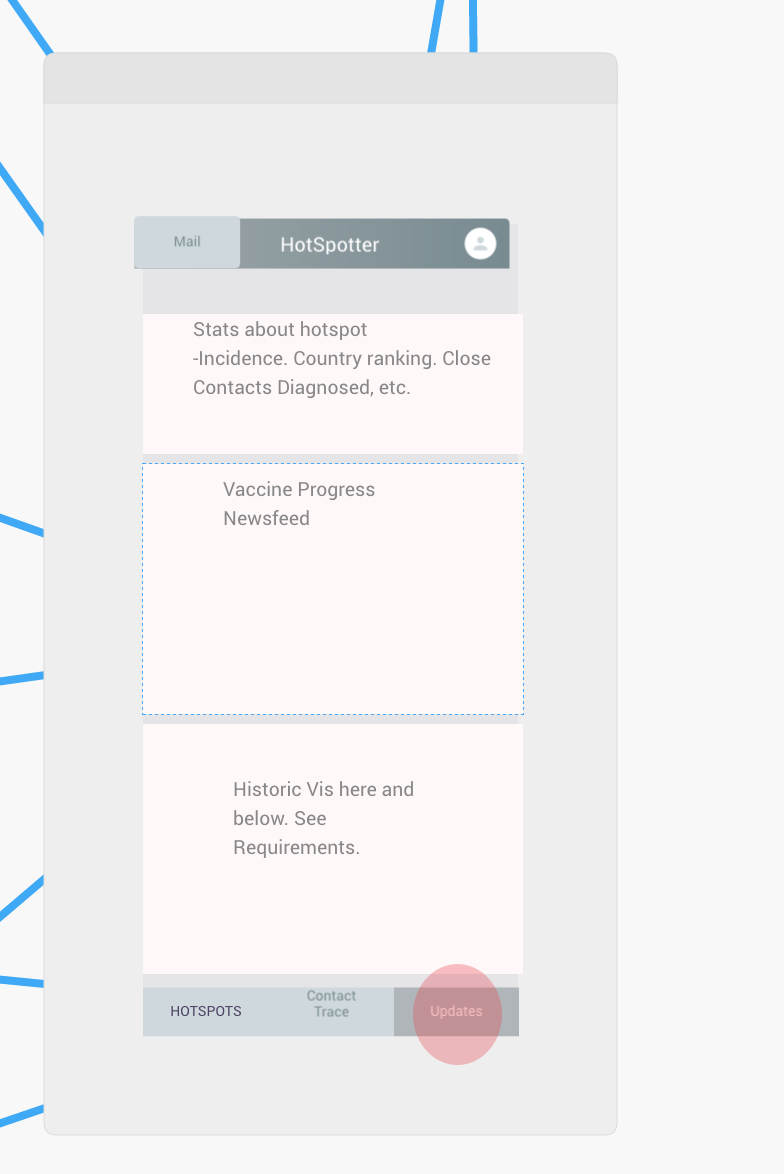
\includegraphics[page=1, width=0.9\linewidth]{COMP30830-Updates}
	\caption{Settings - Consent}
	\label{Updates}
\end{figure}



\begin{figure}[H]
	\centering
	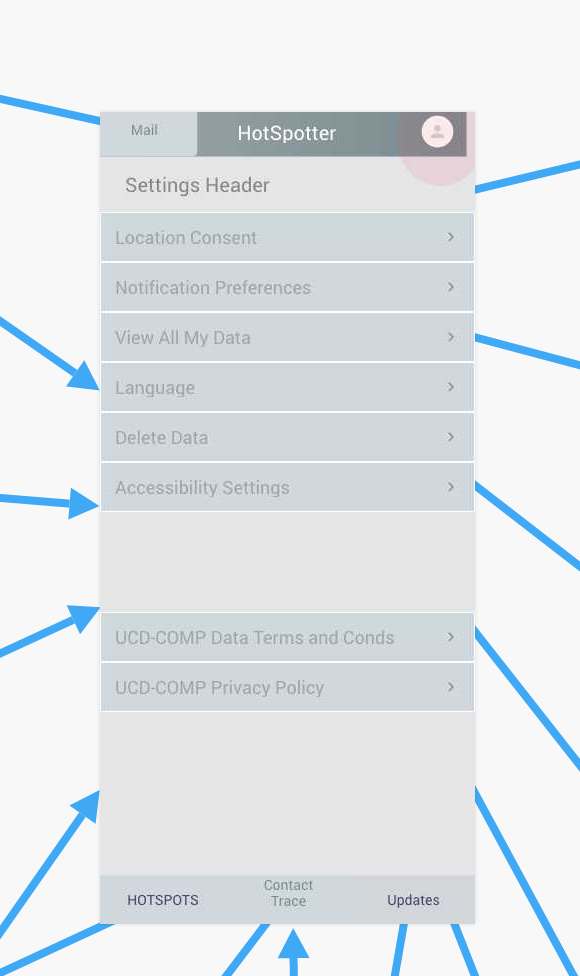
\includegraphics[page=1, width=0.9\linewidth]{COMP30830-Settings}
	\caption{Main Page - Settings}
	\label{Settings}
\end{figure}

\begin{figure}[H]
	\centering
	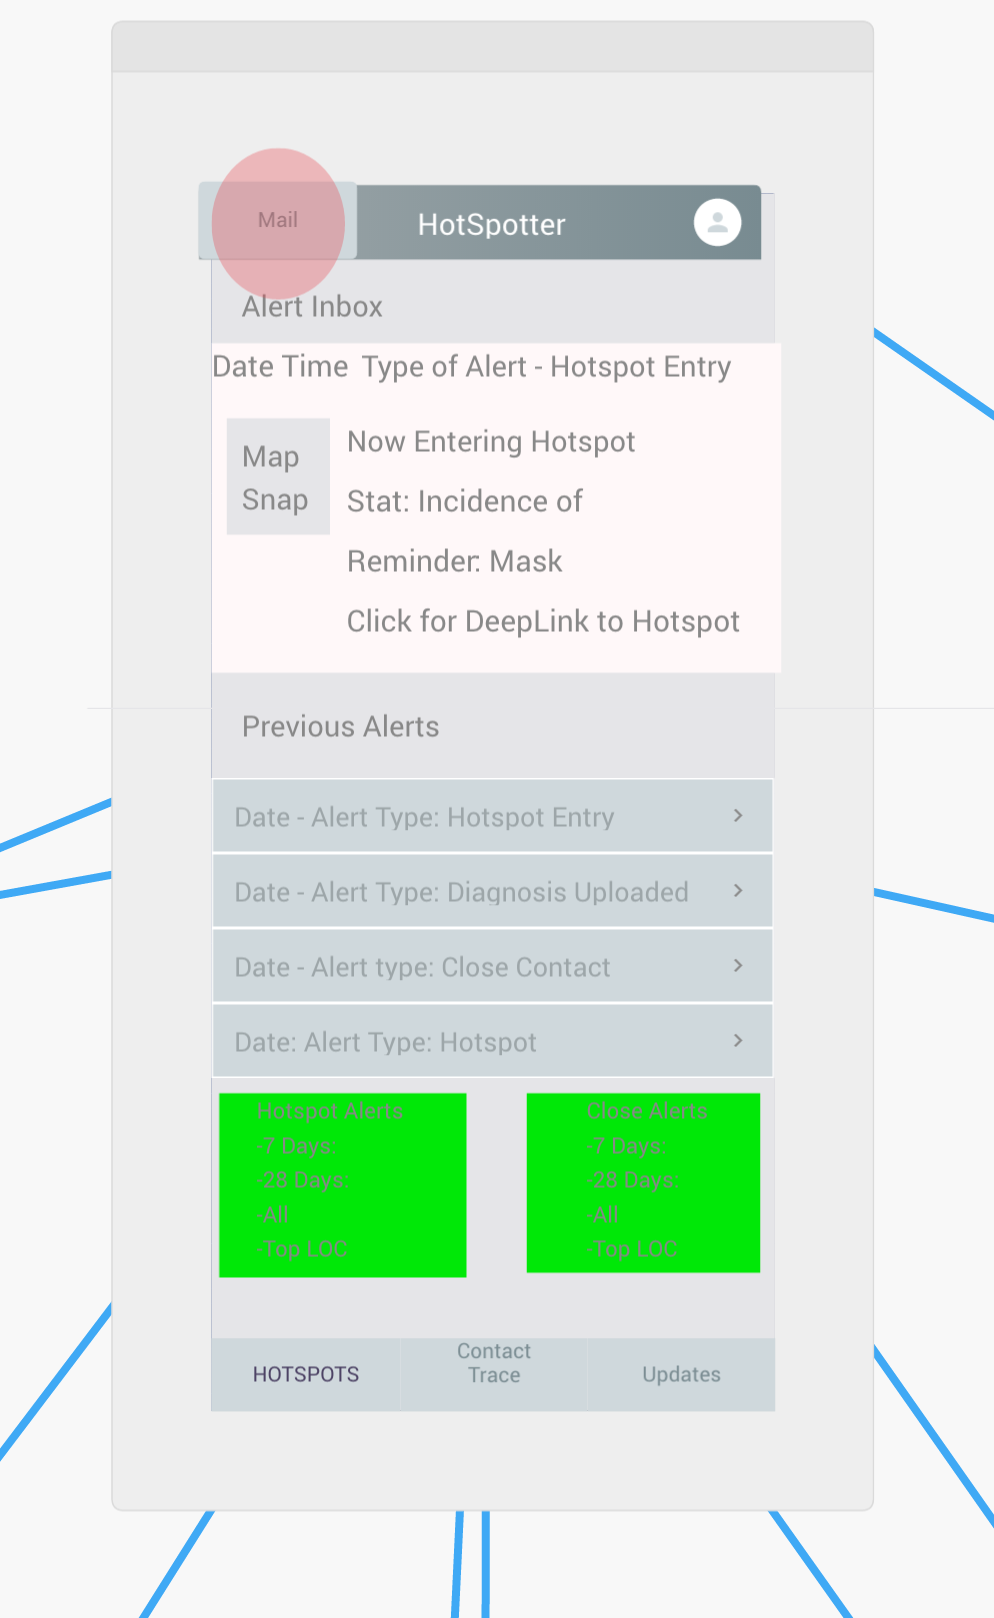
\includegraphics[page=1, width=0.9\linewidth]{COMP30830-Mail}
	\caption{Main Page - Mail}
	\label{Mail}
\end{figure}


\begin{figure}[H]
	\centering
	\includegraphics[page=1, width=0.9\linewidth]{COMP30830-HotSpot-MoreInfo}
	\caption{HotSpot - More Info or Address Search}
	\label{MoreInoHot}
\end{figure}

\begin{figure}[H]
	\centering
	\includegraphics[page=1, width=0.9\linewidth]{COMP30830-Consent}
	\caption{Settings - Location Tracking Consent}
	\label{Consent}
\end{figure}


\begin{figure}[H]
	\centering
	\includegraphics[page=1, width=0.9\linewidth]{COMP-30830-Notification}
	\caption{Settings - Notification Consent}
	\label{Notification}
\end{figure}

\begin{figure}[H]
	\centering
	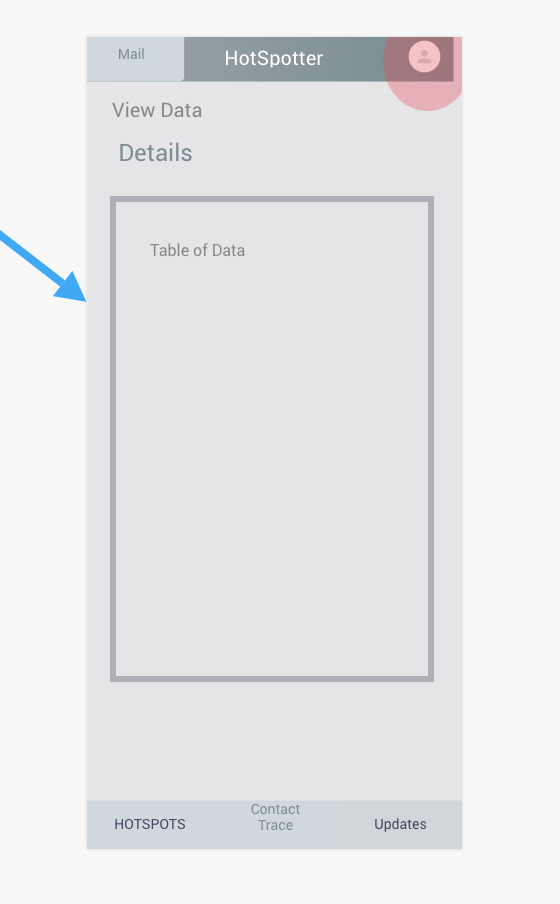
\includegraphics[page=1, width=0.9\linewidth]{COMP30830-Table}
	\caption{Settings - GDPR - Right to Retrieval}
	\label{Table}
\end{figure}


\begin{figure}[H]
	\centering
	\includegraphics[page=1, width=0.9\linewidth]{COMP30830-Language}
	\caption{Settings - Language Options}
	\label{Language}
\end{figure}


\begin{figure}[H]
	\centering
	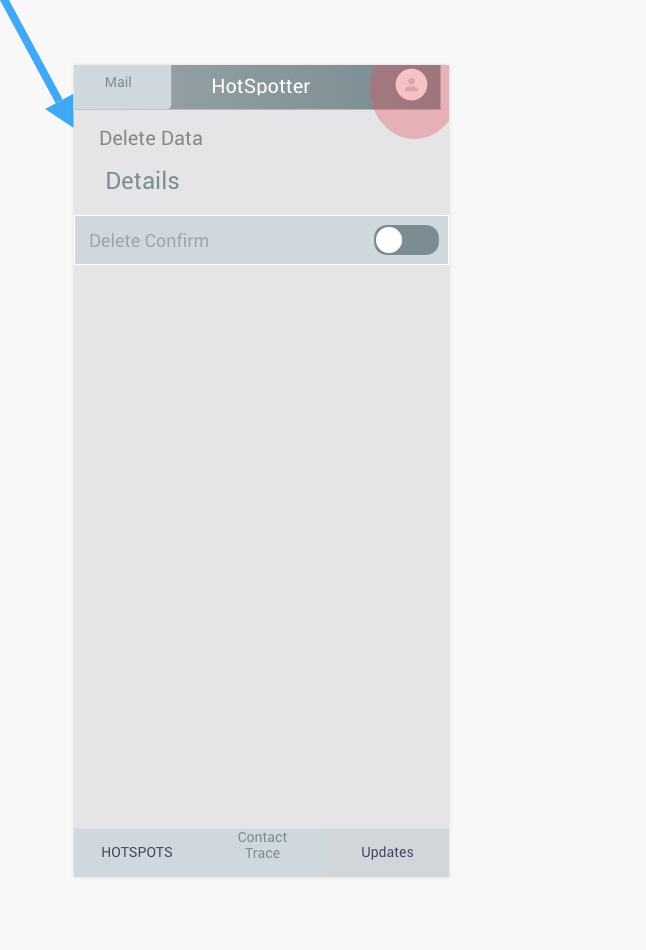
\includegraphics[page=1, width=0.9\linewidth]{COMP30830-DeleteData}
	\caption{Settings - Right to be Forgotten}
	\label{Delete}
\end{figure}


\begin{figure}[H]
	\centering
	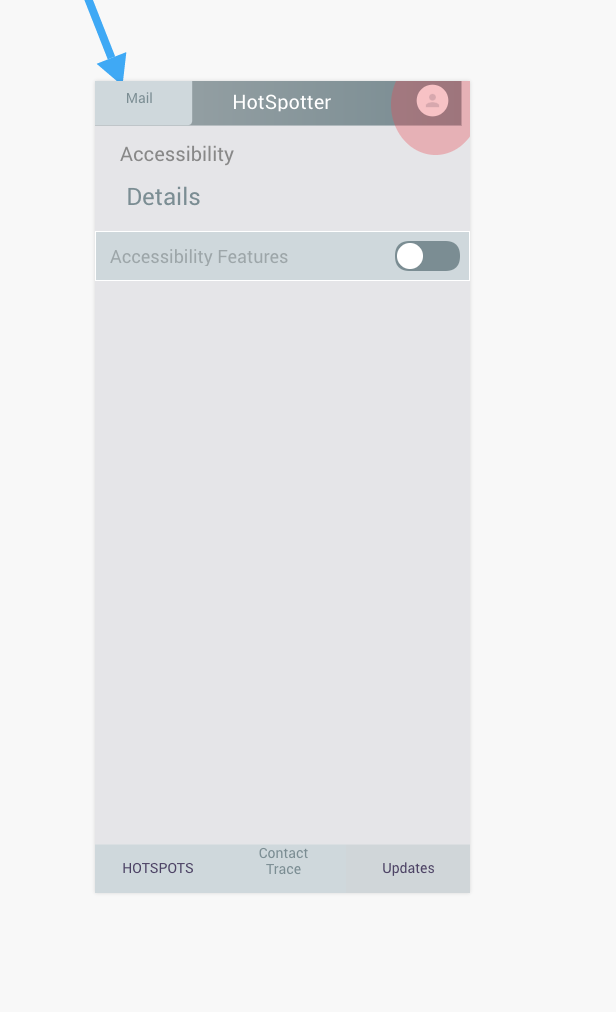
\includegraphics[page=1, width=0.9\linewidth]{COMP30830-Accessibility}
	\caption{Settings - Accessibility}
	\label{Access}
\end{figure}

\end{document}
